\chapter{Validation Test Cases}
\label{cha:tests}


\section{Introduction}

In order to validate the coupling adapter developed in this work, a set of test cases have been simulated, which are supposed to qualitatively and quantitatively confirm the physically correctness of the implementation.

The validation has been carried out in different steps: the first task (section \ref{sec:dummy}) consisted in validating the MBDyn model that has been used throughout the simulations and verifying that the implementation of the coupling works as expected.

The second step aimed at comparing the results obtained performing an FSI simulation with MBDyn with another structural solver, both in compressible and in incompressible regime (Sections \ref{sec:cx-mbd} and \ref{sec:su2-mbd}).

Then, some results obtained from FSI simulations coupling MBDyn with OpenFOAM, have been compared with some benchmarks present in literature. At first, the problem described in \cite{ramm1998fluid} has been considered (see Section \ref{sec:sq-cyl-bench}): it is composed of a square bluff body with a trailing flap. It is characterized by a mass ratio (see Section \ref{subsec:mass-ratio}) of $1.18\cdot 10^{-3}$, this turned out to be a fundamental parameter fo the convergence of simulations, and has been extensively analyzed in the subsequent sections.

One set of well-known benchmarks in FSI literature are the three Turek-Hron FSI test cases described in \cite{turek2006proposal}. Those cases are characterized by the same domain (a round cylinder with a trailing flap) and the same fluid properties. Changes impact only fluid velocity and structural properties (in particular $\rho,E$).

At first, the so-called FSI2 benchmark (characterized by a mass number of $0.1$) has been considered (Section \ref{sec:FSI2}). This benchmark, together with the previous one, shows the validity of the adapter and its potential use in FSI simulations.

Finally, the FSI3 benchmark has been extensively analyzed (Section \ref{sec:FSI1-FSI3}). It has a mass number of $1$ and, up to now, it hasn't been possible to find a suitable set of coupling parameters that can make this case converge when coupled with MBDyn.

It appears that the added mass effect (see Section \ref{sec:added-mass}), plays a dominant role in the convergence of a FSI problems with MBDyn. For this reason, a sensitivity analysis has been performed on the FSI3 problem setup (Section \ref{sec:FSI3-sensitivity}). In particular, flow velocity, fluid density and solid stiffness have been varied in order to gain some insight about the range of parameters, and adimensional numbers that must be considered to understand how critical a simulation can be.     

Each section starts with a short description of the test case, including the most relevant parameter: e.g. the fluid domain geometry and discretization, structural and coupling parameters. Finally some results are presented, together with the coupling performances.

The meshes for all test cases have generated with the free software \textit{Salome}\footnote{\href{https://www.salome-platform.org/}{salome-platform.org/}}. Files for MBDyn interface points have been generated by a Python script running within the \textit{Salome} environment. The script is part of the software made for this work. 


\section{Dummy fluid solver}
\label{sec:dummy}

The first task implemented to validate the adapter consisted in developing a simple \textit{dummy fluid solver}: i.e. a software component connected to the coupling library preCICE with the simple task to apply forces to user-defined nodes on the structure and read back the displacements of the interface nodes.

This approach allowed first to validate the MBDyn model with the \texttt{external structural mapping} component (see Section \ref{sec:mbd-forces}) and the correct data exchange between preCICE and the adapter. 

The \textit{dummy solver} has been written in Python and it is part of the software package in this work.

A MBDyn cantilever beam model composed of 5 \texttt{beam3} elements (see Section \ref{sec:mbd-beam}) has been written to perform this test, as depicted in Figure \ref{fig:cnt-beams}. This requires a total of 11 \texttt{node} elements to define the structure.

The beam section is uniform and rectangular ($w \times h$) and the physical properties (eg. $\rho, E, \nu$) are constant throughout the beam length. 

\begin{figure}[htbp!]
	    \centering
        \begin{tikzpicture}
            \point{a}{0}{0};
            \point{b}{1.5}{0};
            \point{c}{3}{0};
            \point{d}{4.5}{0};
            \point{e}{6}{0};
            \point{f}{7.5}{0};
            
            \beam{4}{a}{b};
            \beam{4}{b}{c};
            \beam{4}{c}{d};
            \beam{4}{d}{e};
            \beam{4}{e}{f};
            
            \notation{2}{b}{};
            \notation{2}{c}{};
            \notation{2}{d}{};
            \notation{2}{e}{};
            \notation{2}{f}{};
            
            \notation{4}{a}{b}[ $1$ ];
            \notation{4}{b}{c}[ $2$ ];
            \notation{4}{c}{d}[ $3$ ];
            \notation{4}{d}{e}[ $4$ ];
            \notation{4}{e}{f}[ $5$ ];
            
            \support{3}{a}[-90];
            % \load{1}{b}[90][1][.1];
            
            \dimensioning{1}{a}{f}{-1.8}[$L$];
            \dimensioning{1}{a}{b}{-1}[$l$];
            
            \dscaling{3}{0.5};
            \daxis{1}{-1.5 ,0 ,0}[right][above][left];
        \end{tikzpicture}
    	\caption{cantilever made of 5 beam elements}
		\label{fig:cnt-beams}
\end{figure}

The inertia of the structure is provided by 2 \texttt{body} elements (see Section \ref{sec:mbd-body} attached to the second and third nodes of each beam (see Figure \ref{fig:mbdyn-beam-model}). The center of gravity of each body is offset by $-l/4$ in x-direction (where $l$ is the length of the single beam element). Each body has the following inertial properties (see Figure \ref{fig:cnt-mass}): 

\begin{equation}
    m = \rho wh \frac{l}{4} \quad I = \frac{m}{12} \begin{bmatrix} h^2+w^2 & 0 & 0 \\ 0 & \frac{l^2}{16} + w^2 & 0 \\ 0 & 0 & \frac{l^2}{16} + h^2 \end{bmatrix}
    \label{eq:body-inertia}
\end{equation}


\begin{figure}[htbp!]
	    \centering
\begin{tikzpicture}[every edge quotes/.append style={auto, text=blue}]
  \pgfmathsetmacro{\cubex}{4}
  \pgfmathsetmacro{\cubey}{2}
  \pgfmathsetmacro{\cubez}{3}
  \draw [draw=blue, every edge/.append style={draw=blue, densely dashed, opacity=.5}, fill=yellow!10]
    (0,0,0) coordinate (o) -- ++(-\cubex,0,0) coordinate (a) -- ++(0,-\cubey,0) coordinate (b) edge coordinate [pos=1] (g) ++(0,0,-\cubez)  -- ++(\cubex,0,0) coordinate (c) -- cycle
    (o) -- ++(0,0,-\cubez) coordinate (d) -- ++(0,-\cubey,0) coordinate (e) edge (g) -- (c) -- cycle
    (o) -- (a) -- ++(0,0,-\cubez) coordinate (f) edge (g) -- (d) -- cycle;
  \path [every edge/.append style={draw=black, |-|}]
    (b) +(0,-5pt) coordinate (b1) edge ["$l/2$"] (b1 -| c)
    (b) +(-5pt,0) coordinate (b2) edge ["h"] (b2 |- a)
    (c) +(3.5pt,-3.5pt) coordinate (c2) edge ["w"] ([xshift=3.5pt,yshift=-3.5pt]e)
    ;
    \daxis{1} {-8,-1,-1.5} [right][above][left];
    \dpoint{q}{-2.5}{-1}{-1.5};
    \dpoint{r}{0}{-1}{-1.5};
    \dpoint{s}{-\cubex}{-1}{-1.5};
    \dpoint{t}{\cubex}{-1}{-1.5};
    \beam{4}{q}{r};
    \dhinge{1}{q};
    \dhinge{1}{r};
    \dhinge{1}{s};
    \dhinge{1}{t};
    \dnotation{1}{q}{CoG};
    \dnotation{1}{r}{$n_2$};
    \dnotation{1}{s}{$n_1$};
    \dnotation{1}{t}{$n_3$};
    \ddimensioning{xy}{q}{r}{1.5}[ $l/4$ ];
    \ddimensioning{xy}{s}{t}{-2.5}[ $l$ ];
    
\end{tikzpicture}
    	\caption{\texttt{body} element attached to node 2 of the \texttt{beam} element}
		\label{fig:cnt-mass}
\end{figure}


The first node of the structure is clamped (to implement the cantilever constraint), while all other joints are constrained to move in the $x-y$ plane and rotate only around the $x-axis$ so that the structure can move only in the $x-y$ plane.
The interface mesh is represented in Figure \ref{fig:mbdyn-mesh}. Only the connectivity elements belonging to the $x-z$ and $y-z$ plane are represented, but it does not affect the behavior if the structure.


\begin{figure}[htbp!]
	\centering
	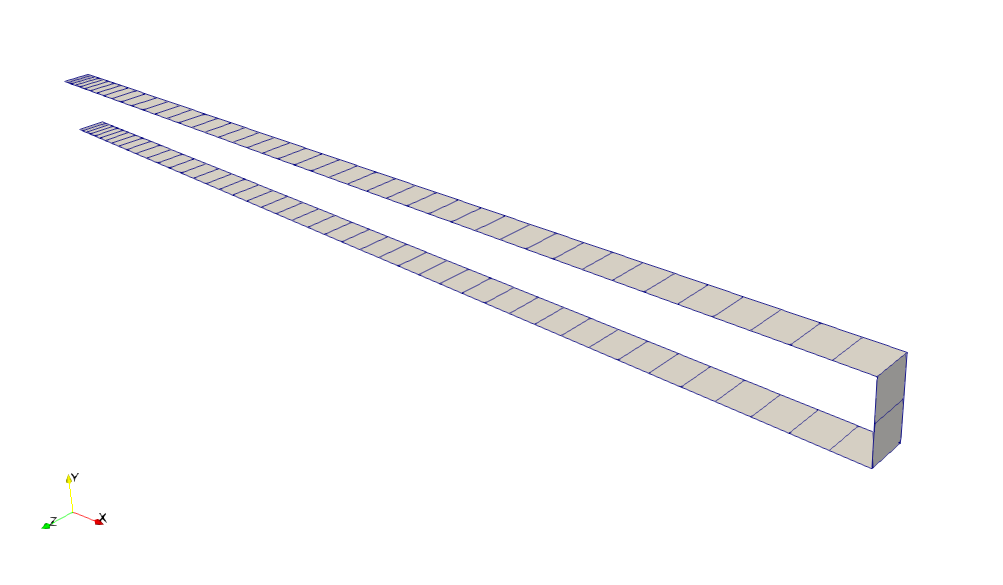
\includegraphics[width=0.7\textwidth]{images/example-mesh}
	\caption{interface points mesh}
	\label{fig:mbdyn-mesh}
\end{figure}

The model has been loaded by a concentrated load on two tip nodes (Figure \ref{fig:cnt-tip}) and with an equivalent distributed load on the nodes belonging to the upper surface (Figure \ref{fig:cnt-distrib}).

\begin{figure}[htbp!]
	%\centering
	    \begin{subfigure}{.8\textwidth}
	    \centering
        \begin{tikzpicture}
            \point{a}{0}{0};
            \point{b}{6}{0};
            \beam{4}{a}{b};
            \support{3}{a}[-90]
            \load{1}{b}[90][1][.1];
        \end{tikzpicture}
    	\caption{cantilever with tip load}
		\label{fig:cnt-tip}
	    \end{subfigure}
	    %\newline
	    \par\bigskip
	    \begin{subfigure}{.8\textwidth}
		\centering
		\begin{tikzpicture}
            \point{a}{0}{0};
            \point{b}{6}{0};
            \beam{4}{a}{b};
            \support{3}{a}[-90]
            \lineload{1}{a}{b}[1][1];%[force interval];
        \end{tikzpicture}
    	\caption{cantilever with distributed load}
		\label{fig:cnt-distrib}
	    \end{subfigure}
	\caption{model and data exchange test-cases}
\end{figure}

The results have been compared the expected theoretical values in terms of tip displacement at steady state and in terms of frequency of the tip movement when the system has been loaded with a step load.

When both the MBDyn model and the data exchanged through the preCICE interface have been validated, the model has been coupled to a CFD solver.





\section{Vertical flap: incompressible regime}
\label{sec:cx-mbd}

The first validation step consisted in comparing the results obtained with MBDyn with the ones given by another structural solver with the same fluid model. 

For this purpose a simple case of a vertical flap immersed in a flow in incompressible regime, has been considered, borrowing an example given in the preCICE website.

\subsection{Fluid domain}

The fluid domain is represented in Figure \ref{fig:ex1-domain}. The inlet is on the left with uniform flow velocity, the outlet is on the right, while all other boundaries are \textit{no-slip} walls.


\begin{figure}[htbp!]
	\centering
	\begin{tikzpicture}
	    \pgfmathsetmacro{\xa}{-0.1}
	    \pgfmathsetmacro{\xb}{0.1}
		\point{a}{-4}{0};
		\point{b}{\xa}{0};
		\point{c}{\xb}{0};
		\point{d}{8}{0};
		\point{e}{\xa}{1};
		\point{f}{\xb}{1};
		\point{g}{-4}{3};
		\point{h}{8}{3};
		
		\point{i}{-3.5}{0.5};
		
		\beam{2}{a}{b};
		\beam{2}{c}{d};
		\beam{2}{a}{g};
		\beam{2}{d}{h};
		\beam{2}{g}{h};
		\beam{4}{b}{e};
		\beam{4}{e}{f};
		\beam{4}{f}{c};
		
		\dimensioning{1}{g}{h}{3.5}[$20m$];
		\dimensioning{1}{a}{b}{-0.6}[$4m$];
		\dimensioning{2}{d}{h}{8.5}[$4m$];
		
		\dimensioning{1}{e}{f}{1.25}[$0.1m$];
		\dimensioning{2}{c}{f}{0.8}[$1m$];
		
		\lineload{1}{a}{g};
		
		\load{1}{i}[180][1][-1];
		\load{1}{i}[-90][1][-1];
		\notation{1}{-2.5,0.25}{x};
		\notation{1}{-3.75,1.5}{z};
		%\dscaling{3}{0.4};
		%\daxis{1}{1.5 ,0 ,0}[right]][above];
	\end{tikzpicture}
	\caption{vertical flap: fluid domain}
	\label{fig:ex1-domain}
\end{figure}


The fluid domain is discretized in an structured hexaedral mesh as depicted in Figure \ref{fig:ex1-mesh}. The main fluid and mesh values are given in Table \ref{table:ex1-fluid} and \ref{table:ex1-mesh}. 

\begin{figure}[htbp!]
	\centering
	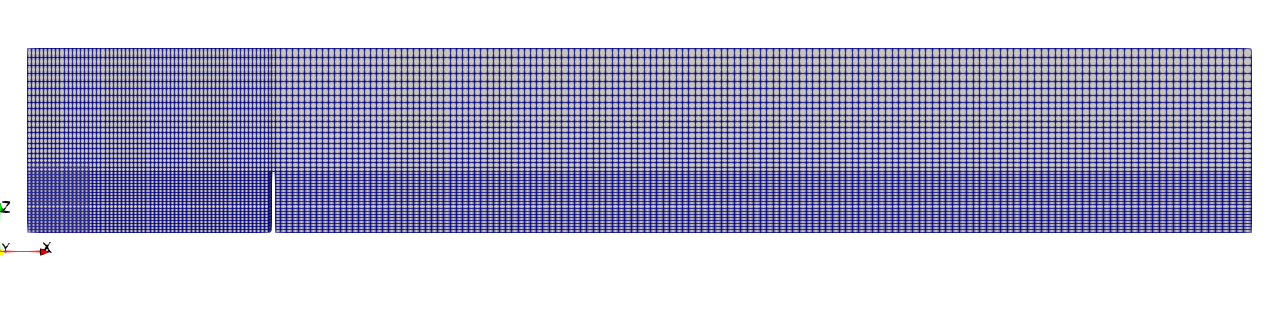
\includegraphics[width=0.9\textwidth]{images/ex1-mesh1}
	\caption{vertical flap: fluid mesh}
	\label{fig:ex1-mesh}
\end{figure}


\begin{table}[!htb]
	\begin{center}
		\begin{tabular}{ l c l | c } 
			parameter & & & value  \\ 
			\hline
			fluid density  & $\rho$ & \si{kg.m^{-3}} & 1   \\
			kinematic viscosity & $\nu$& \si{m^2.s^{-1}} & $10^{-3}$  \\
%			Reynolds length & $l_{Re}$ & $0.1$ & \si{m} \\
%			Reynolds number & Re & $\approx 1000$ & \\
			flow velocity & $\vec{v}$& \si{m.s^{-1}} & 10 \\
			flow type & & & laminar \\
		\end{tabular}
	\end{center}
	\caption{Vertical flap: fluid properties}
	\label{table:ex1-fluid}
\end{table}



\begin{table}[!htb]
	\begin{center}
		\begin{tabular}{ l c | c } 
			parameter & & value   \\ 
			\hline
			number of mesh points  & $n_{dof}$ & 17344     \\
			number of cells & $n_c$ & 8400  \\
			number of interface cells  & $n_{int}$ & 42  \\			
		\end{tabular}
	\end{center}
	\caption{Vertical flap: mesh properties}
	\label{table:ex1-mesh}
\end{table}



\subsection{Simulation and Coupling parameters}

The coupling between the fluid solver and the structural solver is the same for the MBDyn and the CalculiX simulation. The main data are given in Table \ref{table:ex1-coupling}:


\begin{table}[!htb]
	\begin{center}
		\begin{tabular}{ l c  l| c } 
			parameter & & & value   \\ 
			\hline
			simulation time  & $t$& \si{s} & 5      \\
			step size & $\Delta t$ & \si{s} & $10^{-2}$   \\
			\hline
			coupling scheme & & & serial implicit  $S\rightarrow F$  \\
			coupling algorithm & & &  IQN-ILS  \\
			displacement rel. convergence limit & & & $10^{-4}$ \\
			force rel. convergence limit &&  & $10^{-3}$  \\
      		interface mesh mapping & & & RBF  \\
			
		\end{tabular}
	\end{center}
	\caption{Vertical flap: coupling parameters}
	\label{table:ex1-coupling}
\end{table}





\subsection{Structural Solver: CalculiX}

The structural model built in CalculiX is composed of 40 \textbf{C3D8}\footnote{general purpose linear brick element with 8 nodes} as represented in Figure \ref{fig:cx-mesh}. 

\begin{figure}[htbp!]
	\centering
	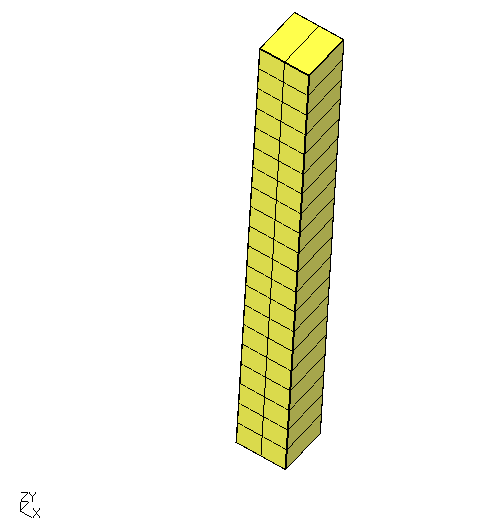
\includegraphics[width=0.6\textwidth]{images/cx1}
	\caption{vertical flap: CalculiX mesh}
	\label{fig:cx-mesh}
\end{figure}

The properties of the solid are reported in Table \ref{table:ex1-solid}.

\begin{table}[!htb]
	\begin{center}
		\begin{tabular}{ l c  l | c } 
			parameter & & value &    \\ 
			\hline
			solid density  & $\rho$ & \si{kg.m^{-3}} & 3000    \\
			Elastic modulus  & E & \si{Pa} & $4\cdot 10^6$    \\
			Poisson coefficient & $\nu$ & & $0.3$  \\
			%			Reynolds length & $l_{Re}$ & $0.1$ & \si{m} \\
			%			Reynolds number & Re & $\approx 1000$ & \\
		\end{tabular}
	\end{center}
	\caption{Vertical flap: solid properties}
	\label{table:ex1-solid}
\end{table}

 
\subsection{Implementation with MBDyn}


The MBDyn model uses the same solid properties of Table \ref{table:ex1-solid} and is composed of 10 \texttt{beam3} elements. Apart from the different orientation, the setup is the same as the one briefly described in Section \ref{sec:dummy}. The only relevant parameter that can be explicitly set up in MBDyn in comparison to CalculiX, consists in the structural damping of the beam elements (see Section \ref{sec:mbd-beam}), which is set to be proportional to stiffness matrix of the element with a coefficient of $2\cdot10^{-3}$.

The interface mesh is divided into 20 faces for the front and back surfaces of the flap. The upper surface is divided into 2, so that the interface is identical to the one obtained in CalculiX. 



\subsection{Results}

The problem considered is characterized by the adimensional parameters given in Table \ref{table:ex1-adim} and its solution is represented in Figure \ref{fig:vf_sol}.


\begin{table}[!htb]
	\begin{center}
		\begin{tabular}{ l c | r } 
			parameter & & value   \\ 
			\hline
			mass number  & $M$ & $3.3\cdot 10^{-4}$     \\
			reduced velocity & $U_R$ & $0.274$  \\
			Cauchy number  & $C_Y$ & $2.5\cdot 10^{-5}$  \\			
		\end{tabular}
	\end{center}
	\caption{Vertical flap: adimensional numbers}
	\label{table:ex1-adim}
\end{table}

\begin{figure}[htbp!]
	\centering
	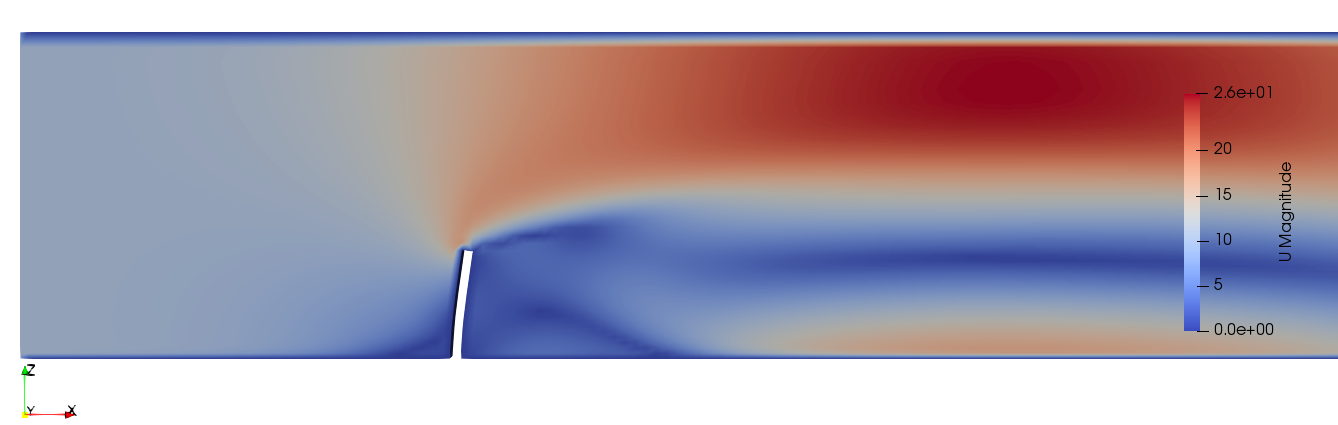
\includegraphics[width=0.9\textwidth]{images/vert_flap/vert_flap1.png}
	\caption{vertical flap: velocity field}
	\label{fig:vf_sol}
\end{figure}


The solutions between CalculiX and MBDyn are first compared in terms of resultants applied to the structure during the simulation (Figures \ref{fig:vf_force} and \ref{fig:vf_moment}), then the tip displacement in $x$ direction is considered in Figure \ref{fig:vf_displacement}. The forces and moments applied to the structure in the two cases are very close. 
The tip displacement shows that both structures exhibit the same damping and the oscillating frequency is very close: CalculiX shows a slightly higher frequency and a more visible second order frequency. The MBDyn structure looks a little more flexible: after 50 seconds of simulation tends to $58mm$ of tip displacement in $x$ direction, while the same structure in CalculiX tends to $53mm$ of displacement. 

\begin{figure}[htbp!]
	\centering
	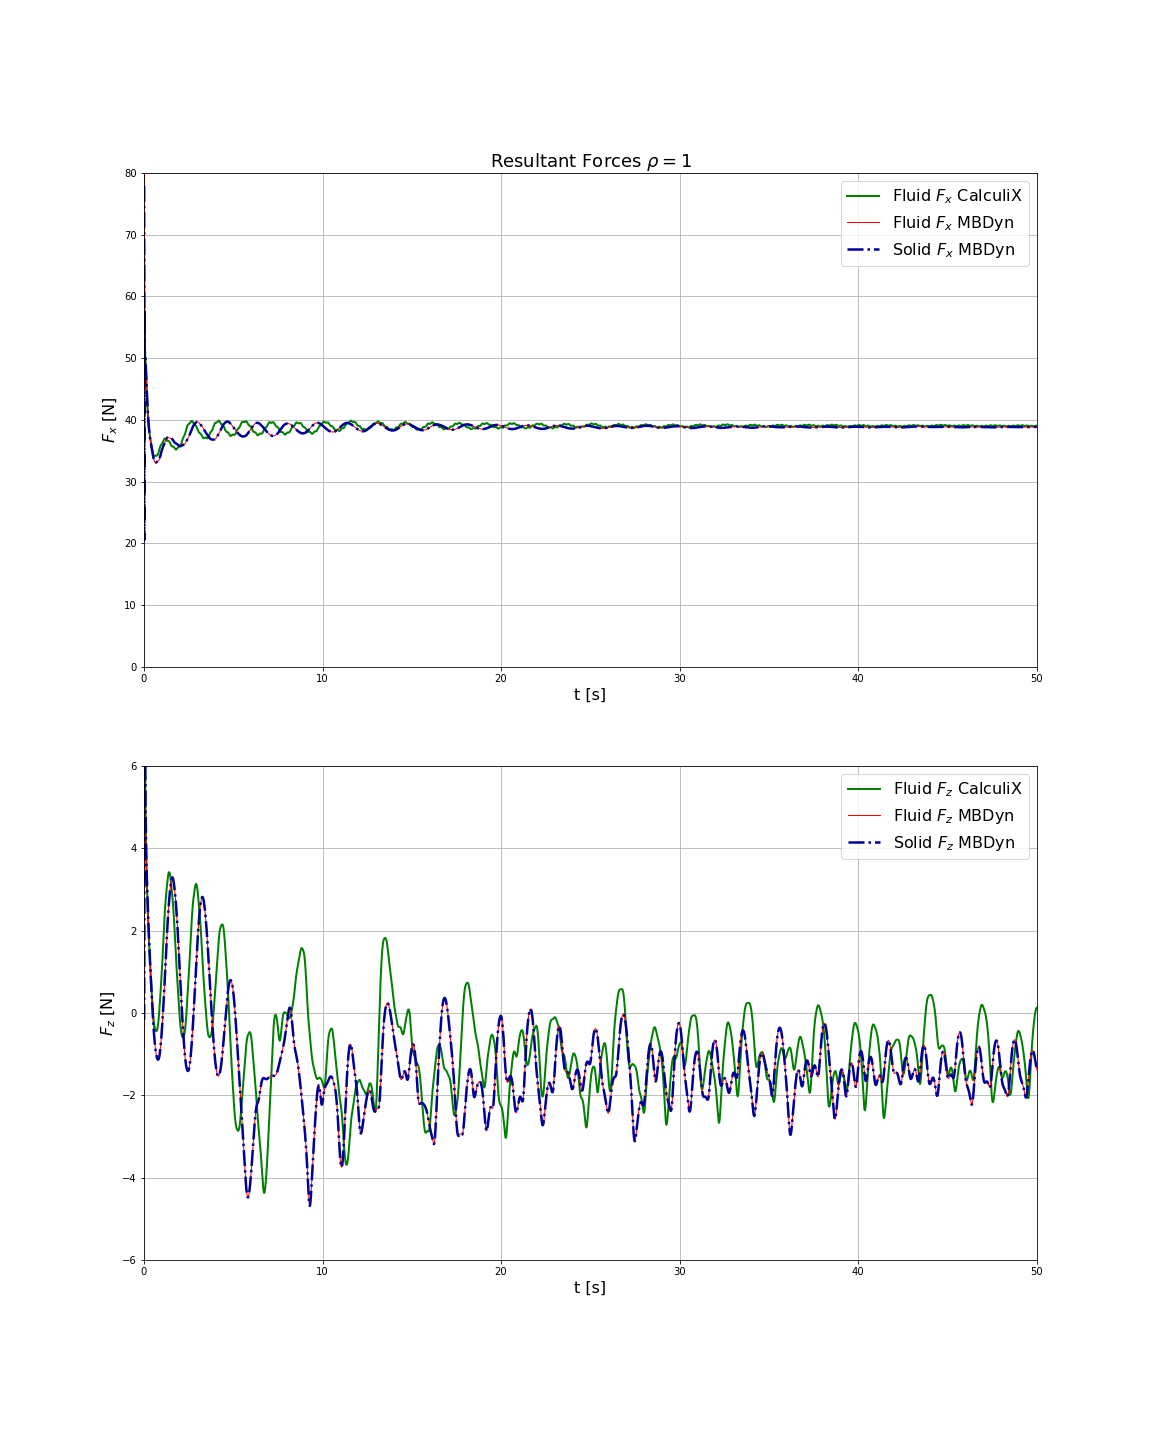
\includegraphics[width=0.9\textwidth]{images/vert_flap/forces_rho1.png}
	\caption{vertical flap: resultant forces}
	\label{fig:vf_force}
\end{figure}

\begin{figure}[htbp!]
	\centering
	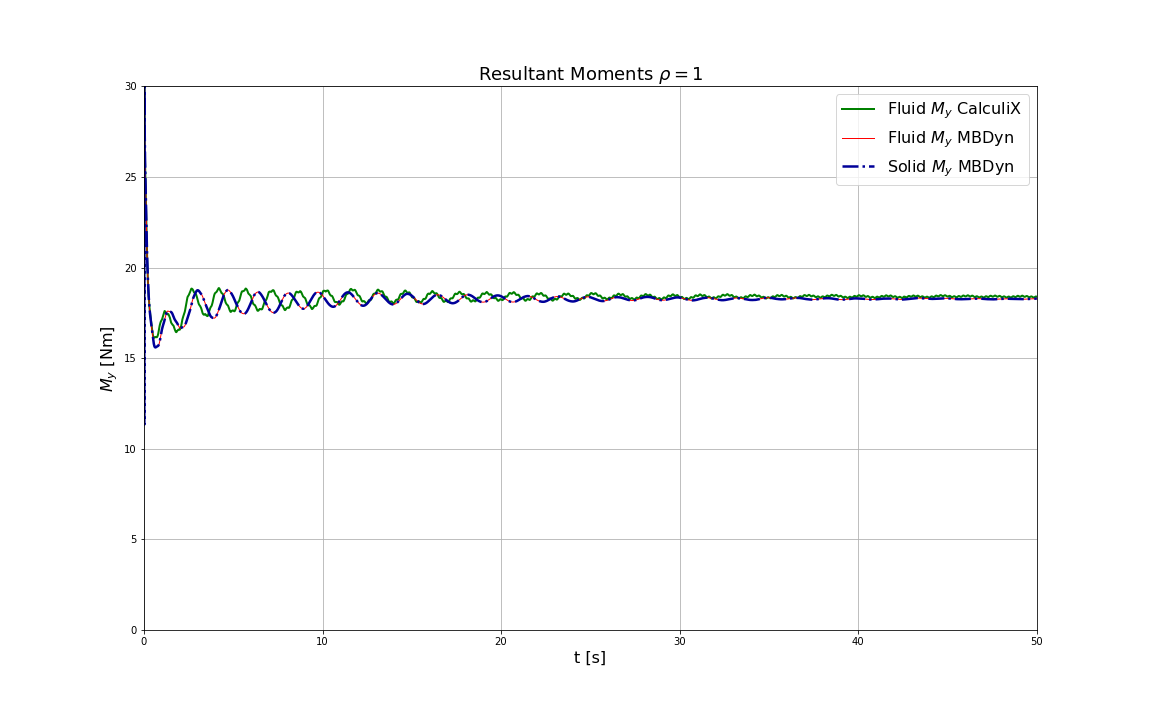
\includegraphics[width=0.9\textwidth]{images/vert_flap/moments_rho1.png}
	\caption{vertical flap: moment applied at root}
	\label{fig:vf_moment}
\end{figure}



\begin{figure}[htbp!]
	\centering
	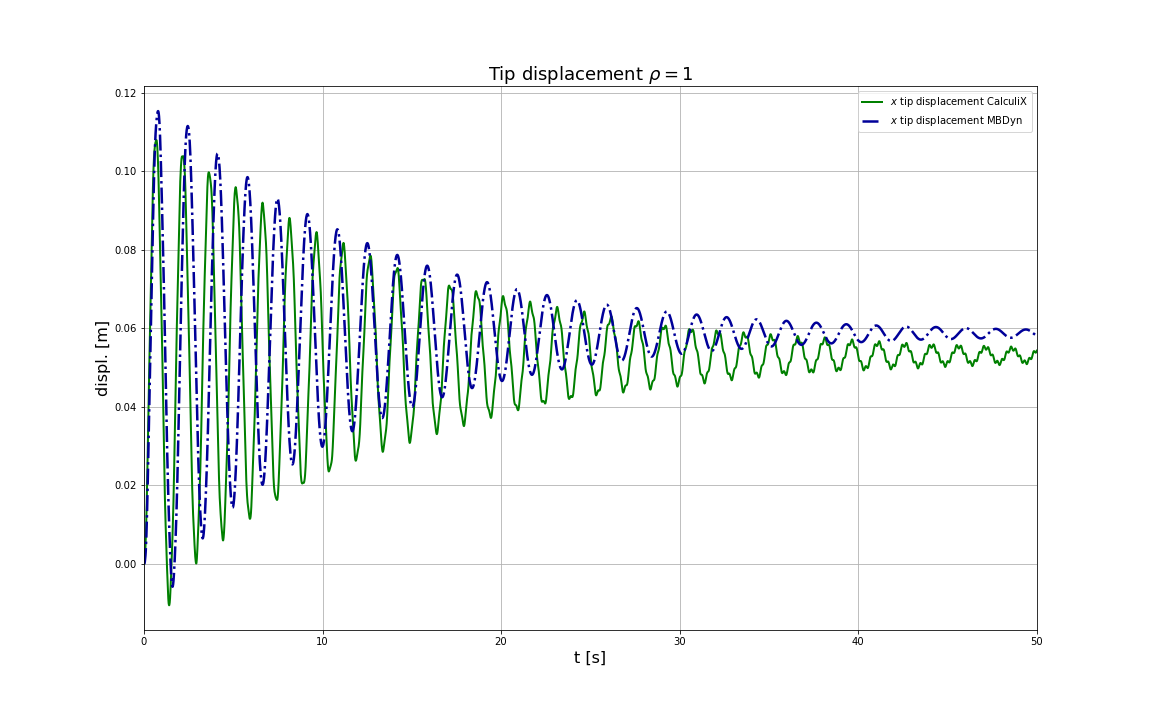
\includegraphics[width=0.9\textwidth]{images/vert_flap/disp_rho1.png}
	\caption{vertical flap: tip displacement x direction}
	\label{fig:vf_displacement}
\end{figure}


As to convergence and number of iterations between the two solvers, Figure \ref{fig:vf_cx_iter} and \ref{fig:vf_mbd_iter} show that, in general, MBdyn and CalculiX require 2 iterations to converge. This can be explained by the small mass number of this case. At some iterations MBDyn requires more iterations: this is due to the fact, for some reasons due to the coupling not completely understood at the moment, a force unbalance arises in the y-direction (out of the plane of the model) which produces a moment around x-axis. This moment is absorbed by the rotation constraints at the nodes and it does not affect the behavior of the resultant in x and z directions. 

\begin{figure}[htbp!]
	\centering
	\begin{subfigure}{0.8\textwidth}
	\centering
	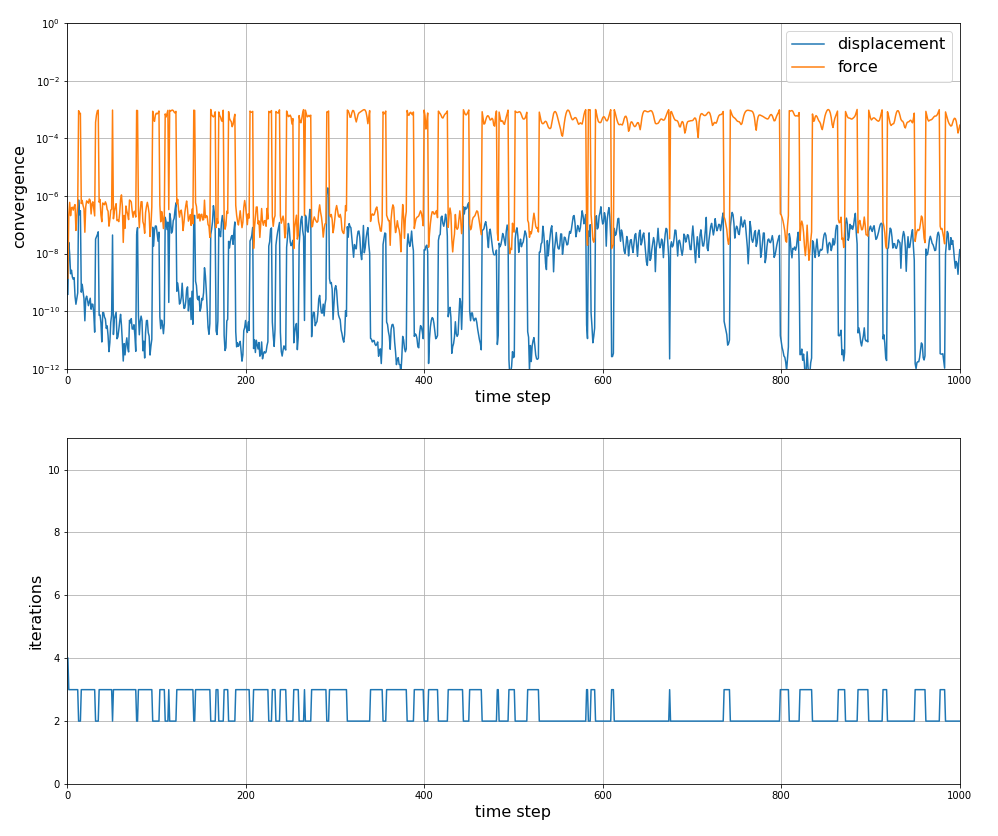
\includegraphics[width=\textwidth, trim=0 0 0 20, clip]{images/vert_flap/CX_iterations_rho1.png}
	\caption{CalculiX}
	\label{fig:vf_cx_iter}
	\end{subfigure}
	\begin{subfigure}{0.9\textwidth}
	\centering
	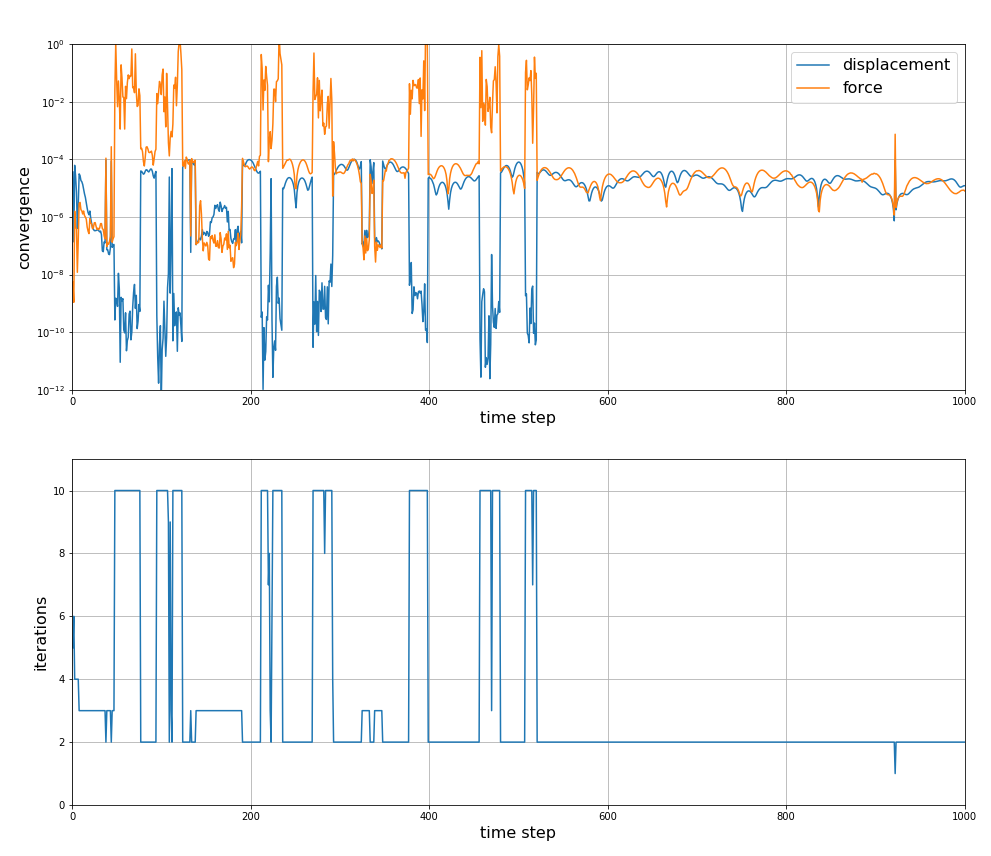
\includegraphics[width=\textwidth, trim=0 0 0 20, clip]{images/vert_flap/MBD_iterations_rho1.png}
	\caption{MBDyn}
	\label{fig:vf_mbd_iter}
	\end{subfigure}
	\caption{vertical flap: convergence and iterations}
	\label{fig:vf_iter}
\end{figure}


Finally, MBDyn allows to analyze the internal forces of each beam, as represented in Figure \ref{fig:vf_mbd_internal}.

\begin{figure}[htbp!]
	\centering
	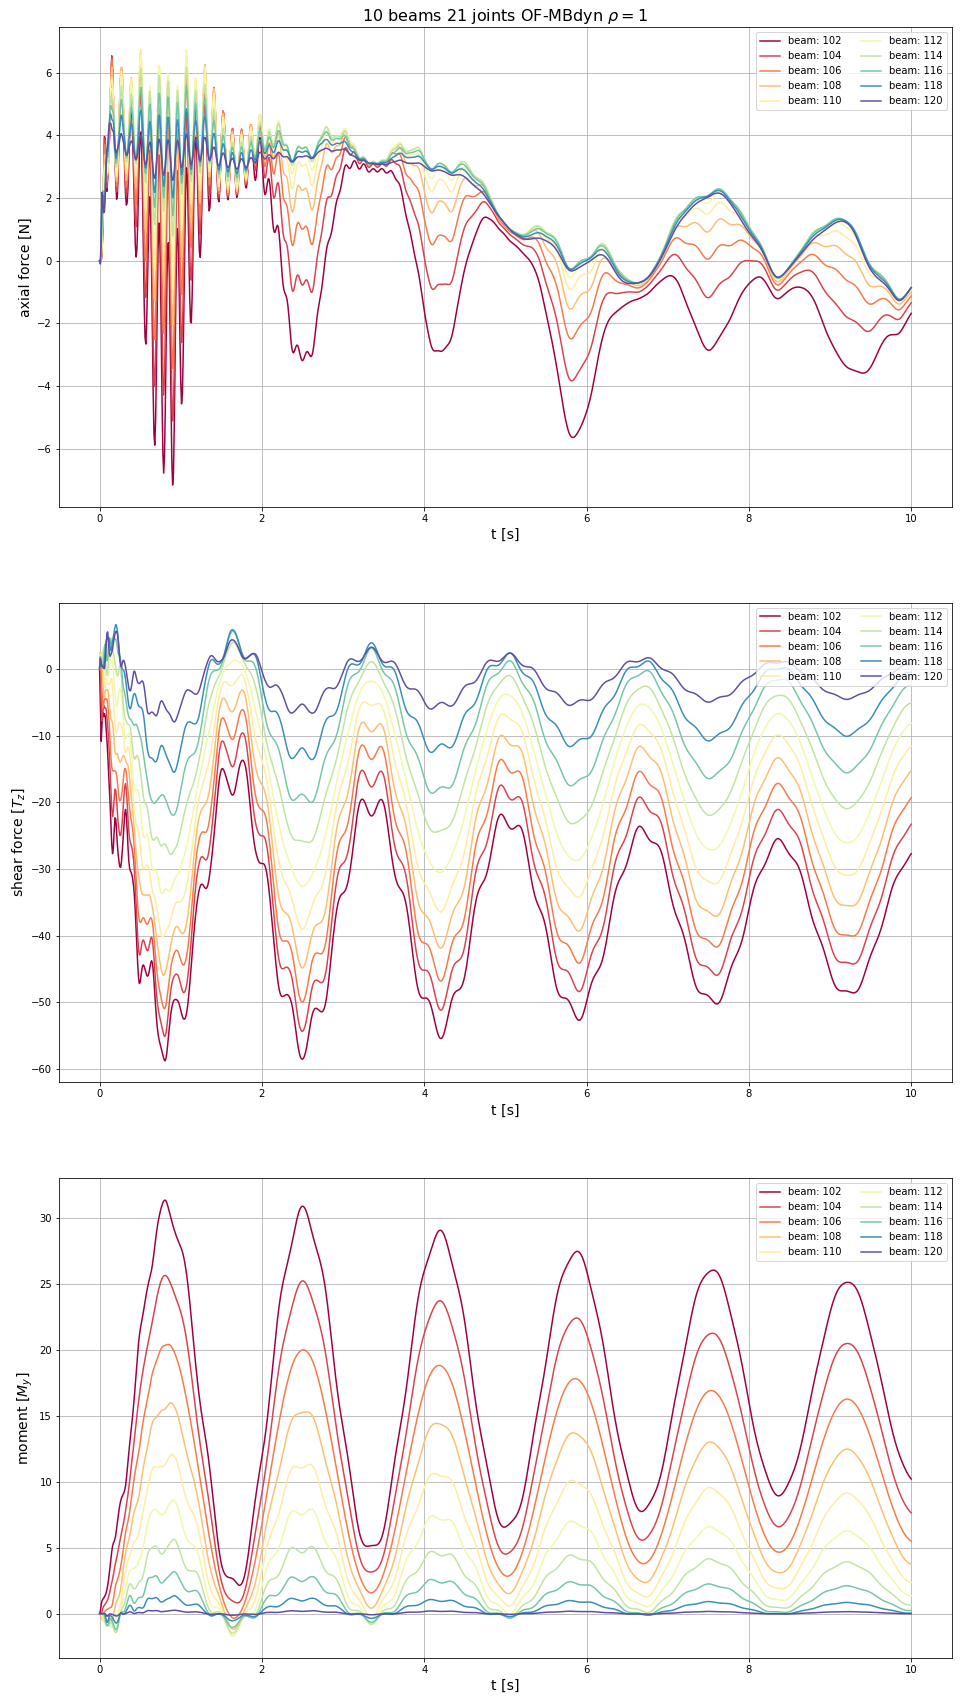
\includegraphics[width=0.82\textwidth]{images/vert_flap/OF-MBDyn_rho1_act.png}
	\caption{vertical flap: MBDyn convergence and iterations}
	\label{fig:vf_mbd_internal}
\end{figure}


\newpage

\section{Vertical flap: compressible regime}
\label{sec:su2-mbd}

A model similar to the one described in the previous section has been used to test the coupling capabilities of the adapter with a different fluid solver: SU2\footnote{\href{https://su2code.github.io/}{su2code.github.io}}. The coupling adapter between SU2 and preCICE allows to build FSI simulations in compressible regime. Besides, SU2 allows to define strictly bidimensional domains, while OpenFOAM and MBDyn are strictly tridimensional. Bidimensionality is enforced in OenFOAM using \textit{empty} boundary conditions, while in MBDyn is enforced through constraints on nodes.
For those reasons a similar model has been built. 


\subsection{Fluid domain}

The fluid domain is represented in Figure \ref{fig:comp-domain}. The inlet is on the left with uniform flow velocity, the outlet is on the right, while all other boundaries are \textit{slip} walls.


\begin{figure}[htbp!]
	\centering
	\begin{tikzpicture}
	    \pgfmathsetmacro{\xa}{-1.1}
	    \pgfmathsetmacro{\xb}{-1}
		\point{a}{-4}{0};
		\point{b}{\xa}{0};
		\point{c}{\xb}{0};
		\point{d}{8}{0};
		\point{e}{\xa}{1};
		\point{f}{\xb}{1};
		\point{g}{-4}{3};
		\point{h}{8}{3};
		
		\point{i}{-3.5}{0.5};
		
		\beam{2}{a}{b};
		\beam{2}{c}{d};
		\beam{2}{a}{g};
		\beam{2}{d}{h};
		\beam{2}{g}{h};
		\beam{4}{b}{e};
		\beam{4}{e}{f};
		\beam{4}{f}{c};
		
		\dimensioning{1}{g}{h}{3.5}[$4.2m$];
		\dimensioning{1}{a}{b}{-0.6}[$1.2m$];
		\dimensioning{2}{d}{h}{8.5}[$1.2m$];
		
		\dimensioning{1}{e}{f}{1.25}[$0.002m$];
		\dimensioning{2}{c}{f}{-0.2}[$0.4m$];
		
		\lineload{1}{a}{g};
		
		\load{1}{i}[180][1][-1];
		\load{1}{i}[-90][1][-1];
		\notation{1}{-2.5,0.25}{x};
		\notation{1}{-3.75,1.5}{y};
		%\dscaling{3}{0.4};
		%\daxis{1}{1.5 ,0 ,0}[right]][above];
	\end{tikzpicture}
	\caption{vertical flap (compressible): fluid domain}
	\label{fig:comp-domain}
\end{figure}


The fluid domain is discretized in an unstructured triangular mesh as depicted in Figure \ref{fig:comp-mesh}. The main fluid and mesh values are given in Table \ref{table:comp-fluid} and \ref{table:comp-mesh}. 

\begin{figure}[htbp!]
	\centering
	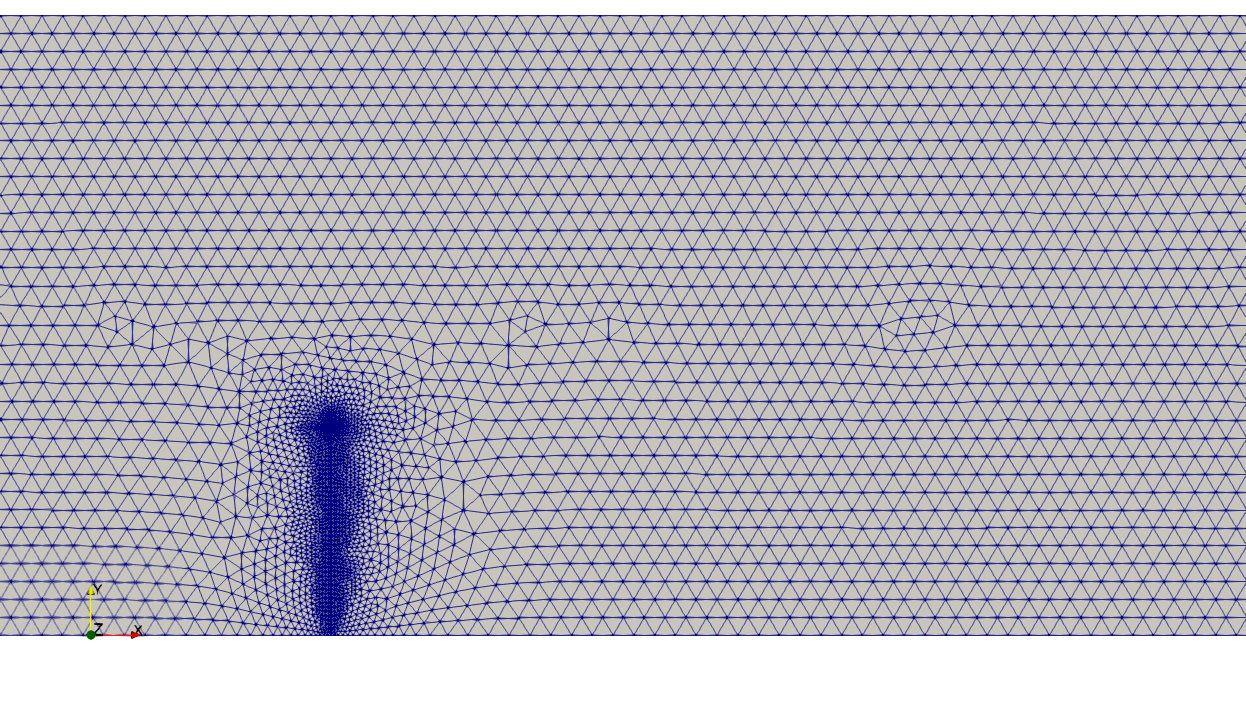
\includegraphics[width=0.9\textwidth, trim=0 100 0 100,clip]{images/comp_flap/mesh.png}
	\caption{vertical flap (compressible): fluid mesh}
	\label{fig:comp-mesh}
\end{figure}


\begin{table}[!htb]
	\begin{center}
		\begin{tabular}{ l c l | c } 
			parameter & & & value  \\ 
			\hline
			fluid properties  &  &  & standard air   \\
			outlet pressure & $p$& \si{Pa} & $101300$  \\
			inlet temperature & $T$ & \si{K} & 288  \\
%			Reynolds number & Re & $\approx 1000$ & \\
			inlet Mach number &  Ma &  & 0.1 \\
			flow type & & & euler \\
		\end{tabular}
	\end{center}
	\caption{Vertical flap (compressible): fluid properties}
	\label{table:comp-fluid}
\end{table}



\begin{table}[!htb]
	\begin{center}
		\begin{tabular}{ l c | c } 
			parameter & & value   \\ 
			\hline
			number of mesh points  & $n_{dof}$ & 5580     \\
			number of cells & $n_c$ & 10709  \\
			number of interface points  & $n_{int}$ & 162  \\			
		\end{tabular}
	\end{center}
	\caption{Vertical flap (compressible): mesh properties}
	\label{table:comp-mesh}
\end{table}


\subsection{MBDyn model}


The MBDyn model uses solid properties defined in Table \ref{table:comp-solid} and is composed of 5 \texttt{beam3} elements. 

\begin{table}[!htb]
	\begin{center}
		\begin{tabular}{ l c  l | c } 
			parameter & & & value   \\ 
			\hline
			solid density  & $\rho$ & \si{kg.m^{-3}} & 1000    \\
			Elastic modulus  & E & \si{Pa} & $ 5.6 \cdot 10^9$    \\
			Poisson coefficient & $\nu$ & & $0.4$  \\
			structural damping & & & $1 \cdot 10^{-3}$ \\
			%			Reynolds length & $l_{Re}$ & $0.1$ & \si{m} \\
			%			Reynolds number & Re & $\approx 1000$ & \\
		\end{tabular}
	\end{center}
	\caption{Vertical flap: solid properties}
	\label{table:comp-solid}
\end{table}

\subsection{Coupling parameters}

The main data concerning the coupling between MBDyn and SU2 are given in Table \ref{table:comp-coupling}:

\begin{table}[!htb]
	\begin{center}
		\begin{tabular}{ l c  l| c } 
			parameter & & & value   \\ 
			\hline
			simulation time  & $t$& \si{s} & 1      \\
			step size & $\Delta t$ & \si{s} & $10^{-3}$   \\
			\hline
			coupling scheme & & & serial implicit $S\rightarrow F$  \\
			coupling algorithm & & &  IQN-ILS  \\
			displacement rel. convergence limit & & & $10^{-5}$ \\
			force rel. convergence limit &&  & $10^{-3}$  \\
      		interface mesh mapping & & & RBF  \\
			
		\end{tabular}
	\end{center}
	\caption{Vertical flap (compressible): coupling parameters}
	\label{table:comp-coupling}
\end{table}


\subsection{Results}

The problem considered is characterized by the adimensional parameters given in Table \ref{table:comp-adim}: in particular the mass number remains in the order of $\mathcal{O} \left(10^{-3}\right)$. A sketch of the flow solution is represented in Figure \ref{fig:comp_sol}.

\begin{table}[!htb]
	\begin{center}
		\begin{tabular}{ l c | r } 
			parameter & & value   \\ 
			\hline
			mass number  & $M$ & $ \approx 1.2\cdot 10^{-3}$     \\
			reduced velocity & $U_R$ & $ \approx 1.44\cdot 10^{-2}$  \\
			Cauchy number  & $C_Y$ & $  \approx 2.53 \cdot 10^{-7}$  \\			
		\end{tabular}
	\end{center}
	\caption{Vertical flap (compressible): adimensional numbers}
	\label{table:comp-adim}
\end{table}

\begin{figure}[htbp!]
	\centering
	\begin{subfigure}{0.9\textwidth}
	\centering
	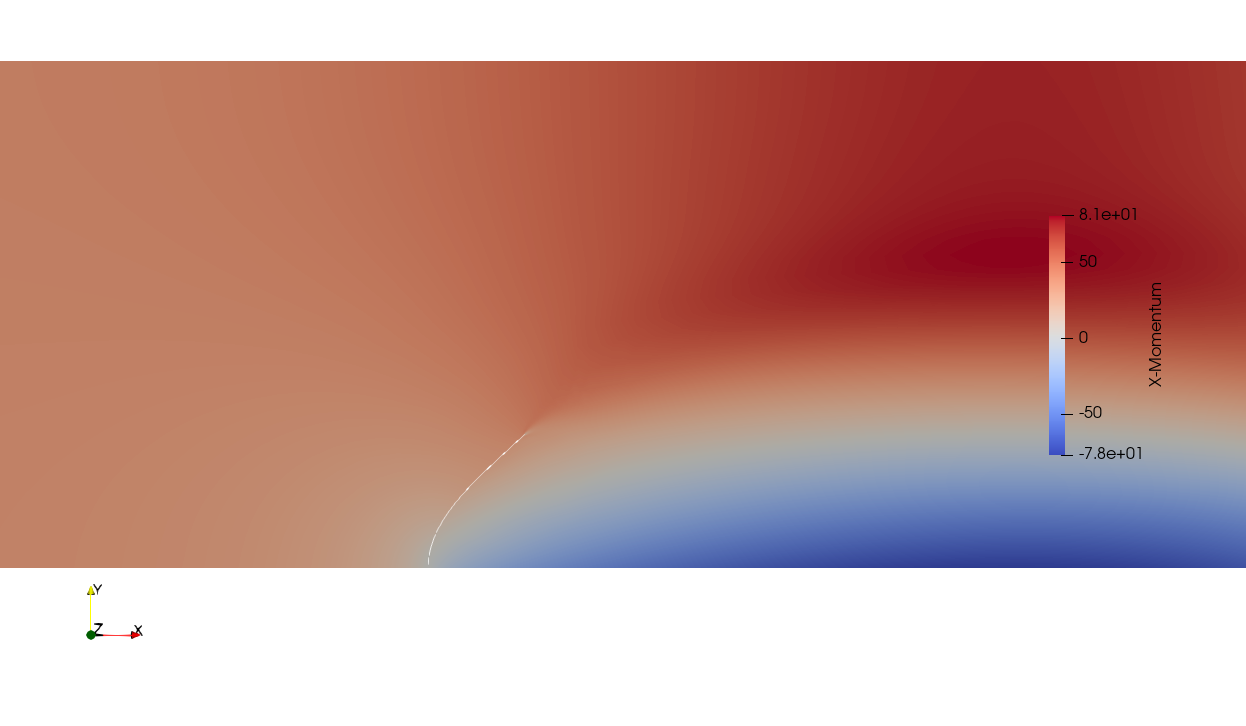
\includegraphics[width=\textwidth, trim=0 150 0 150, clip]{images/comp_flap/x-mom.png}
	\caption{vertical flap (compressible): x-momentum}
	\end{subfigure}
	\begin{subfigure}{\textwidth}
	\centering
	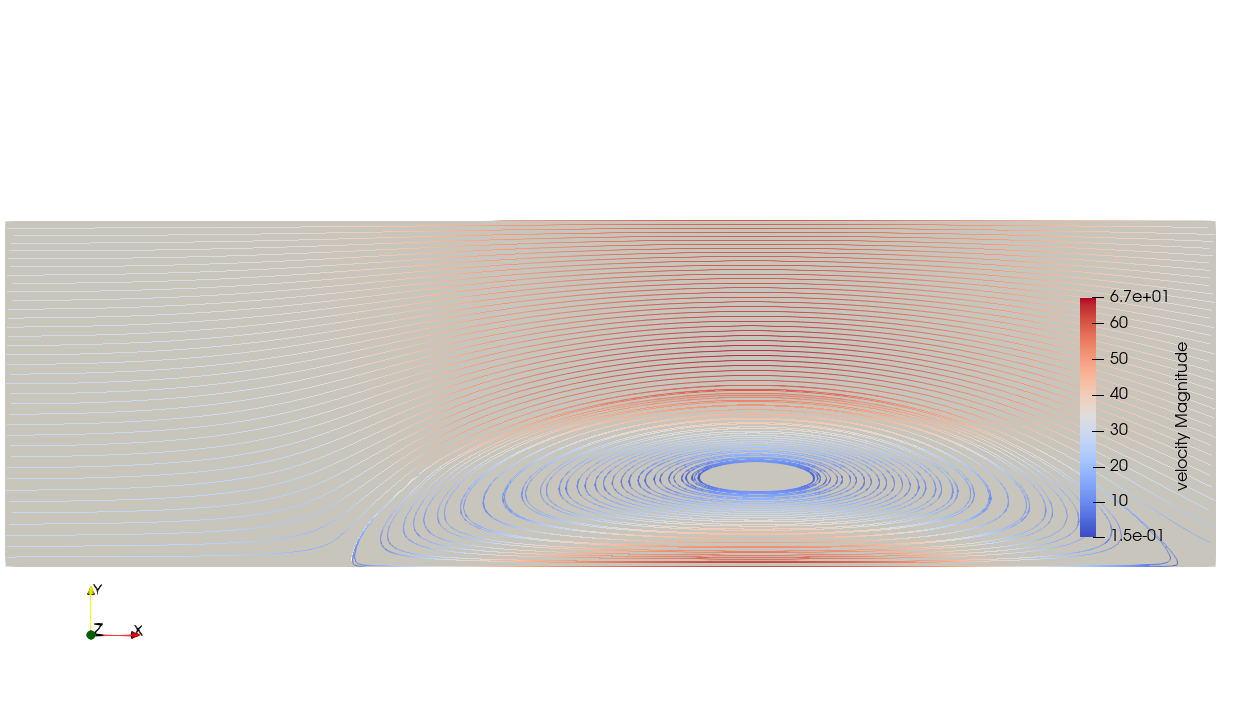
\includegraphics[width=0.95\textwidth, trim=0 150 0 150, clip]{images/comp_flap/vel-stream.png}
	\caption{vertical flap (compressible): streamlines}
	\end{subfigure}
	\caption{vertical flap (compressible): flow solution}
	\label{fig:comp_sol}
\end{figure}


The combination of parameters considered in this test case aimed at considering a very thin flexible element surrounded by a low-Mach flow, so that large displacements are involved. The structure reaches a steady deformed shape after around 1 second as shown in Figure  \ref{fig:comp_displacement}, concerning tip displacement. 

The fluid flow has been initialized with a steady solution obtained considering a rigid structure, then the FSI problem has been simulated applying the the aerodynamic load to the flap progressively: a linear ramp starting at $1\%$ of the load with a duration of 0.2 seconds (see Section \ref{sec:mbdyn-adapter-input} for the adapter input parameters).

Resultant forces $(R_x, R_y)$ and moment $(M_z)$ computed at the root of the flap are shown in Figure \ref{fig:comp_force}.

\begin{figure}[htbp!]
	\centering
	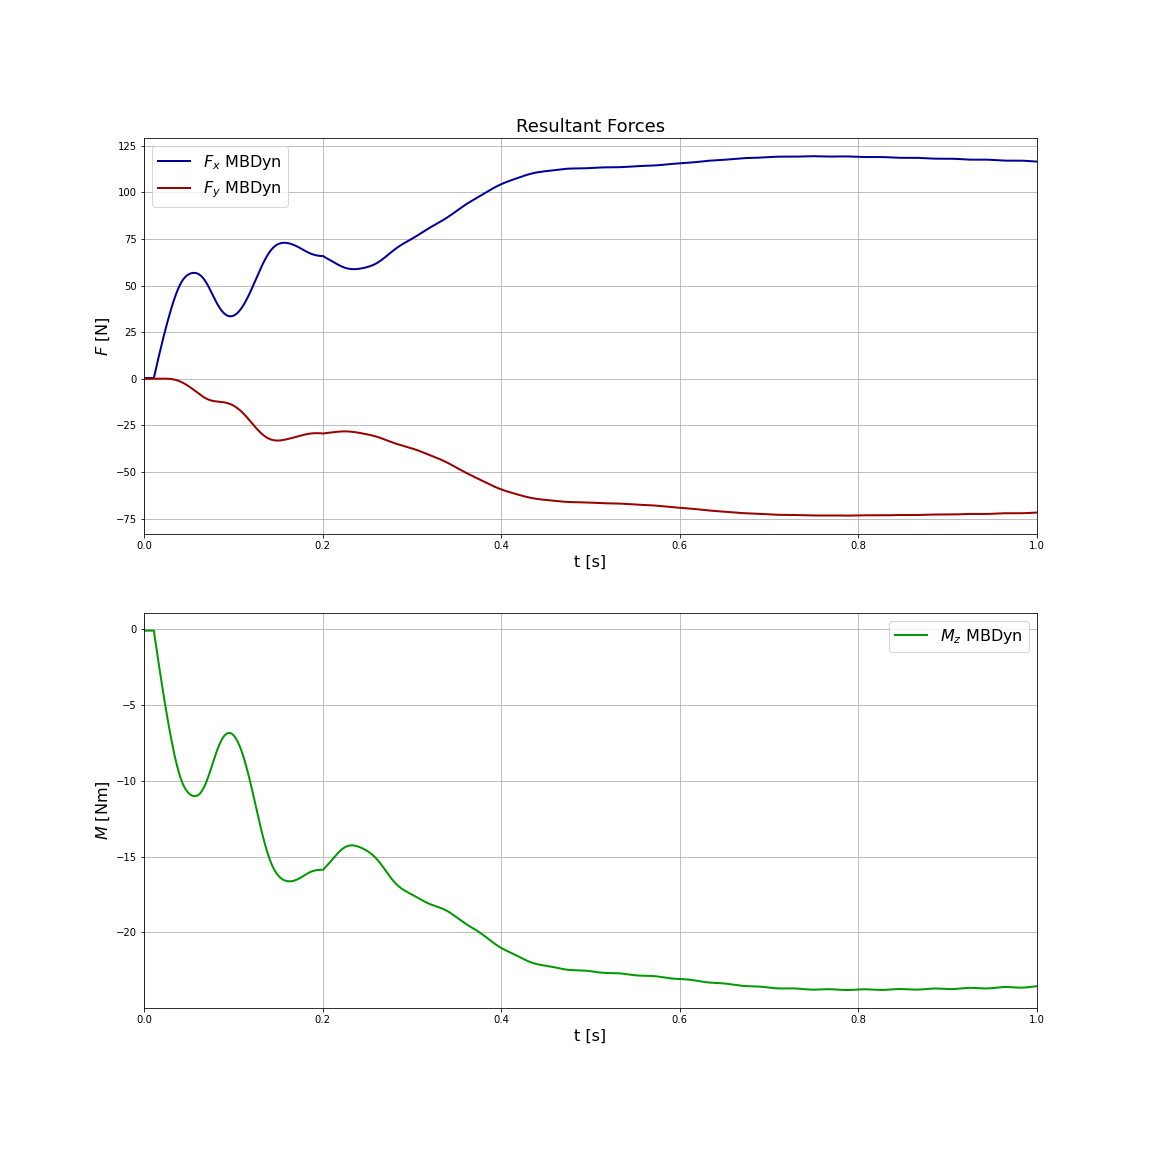
\includegraphics[width=0.9\textwidth, trim=0 100 0 100, clip]{images/comp_flap/forces_comp.png}
	\caption{vertical flap (compressible): resultant forces}
	\label{fig:comp_force}
\end{figure}



\begin{figure}[htbp!]
	\centering
	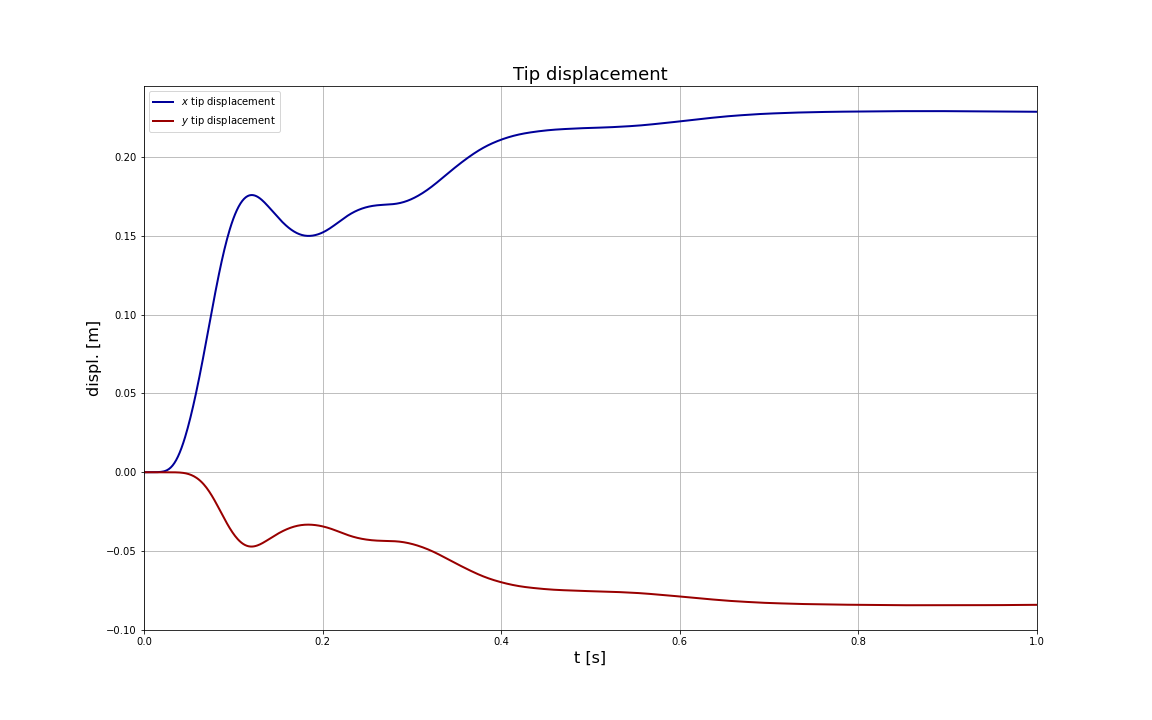
\includegraphics[width=0.9\textwidth, trim=0 50 0 50, clip]{images/comp_flap/disp_comp.png}
	\caption{vertical flap (compressible): tip displacement}
	\label{fig:comp_displacement}
\end{figure}


Each time step of the problem converges quite rapidly, requiring 5 iterations in most cases (see Figure \ref{fig:comp_mbd_iter}. This outcome agrees with the fact that a low mass number and a high fluid velocity make the problem loosely coupled (see section \ref{sec:strong-coupling} for some details). Nevertheless an explicit simulation diverges immediately.  


\begin{figure}[htbp!]
	\centering
	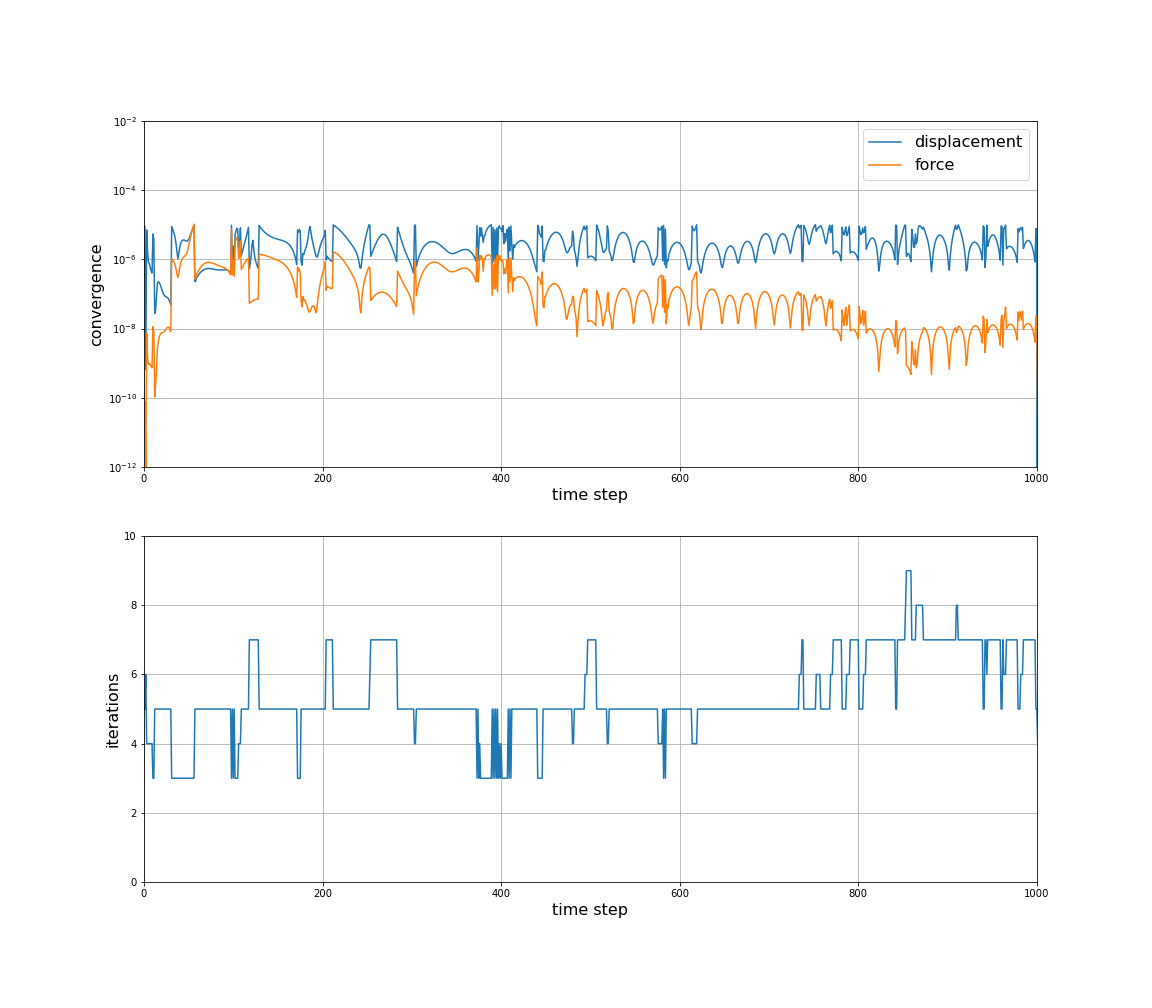
\includegraphics[width=0.95\textwidth, trim=0 80 0 100, clip]{images/comp_flap/MBD_iterations_comp.png}
	\caption{vertical flap (compressible): convergence and iterations}
	\label{fig:comp_mbd_iter}
\end{figure}

Axial, shear and bending moment in each of the MBDyn elements are plotted in Figure \ref{fig:comp_mbd_internal}.

\begin{figure}[htbp!]
	\centering
	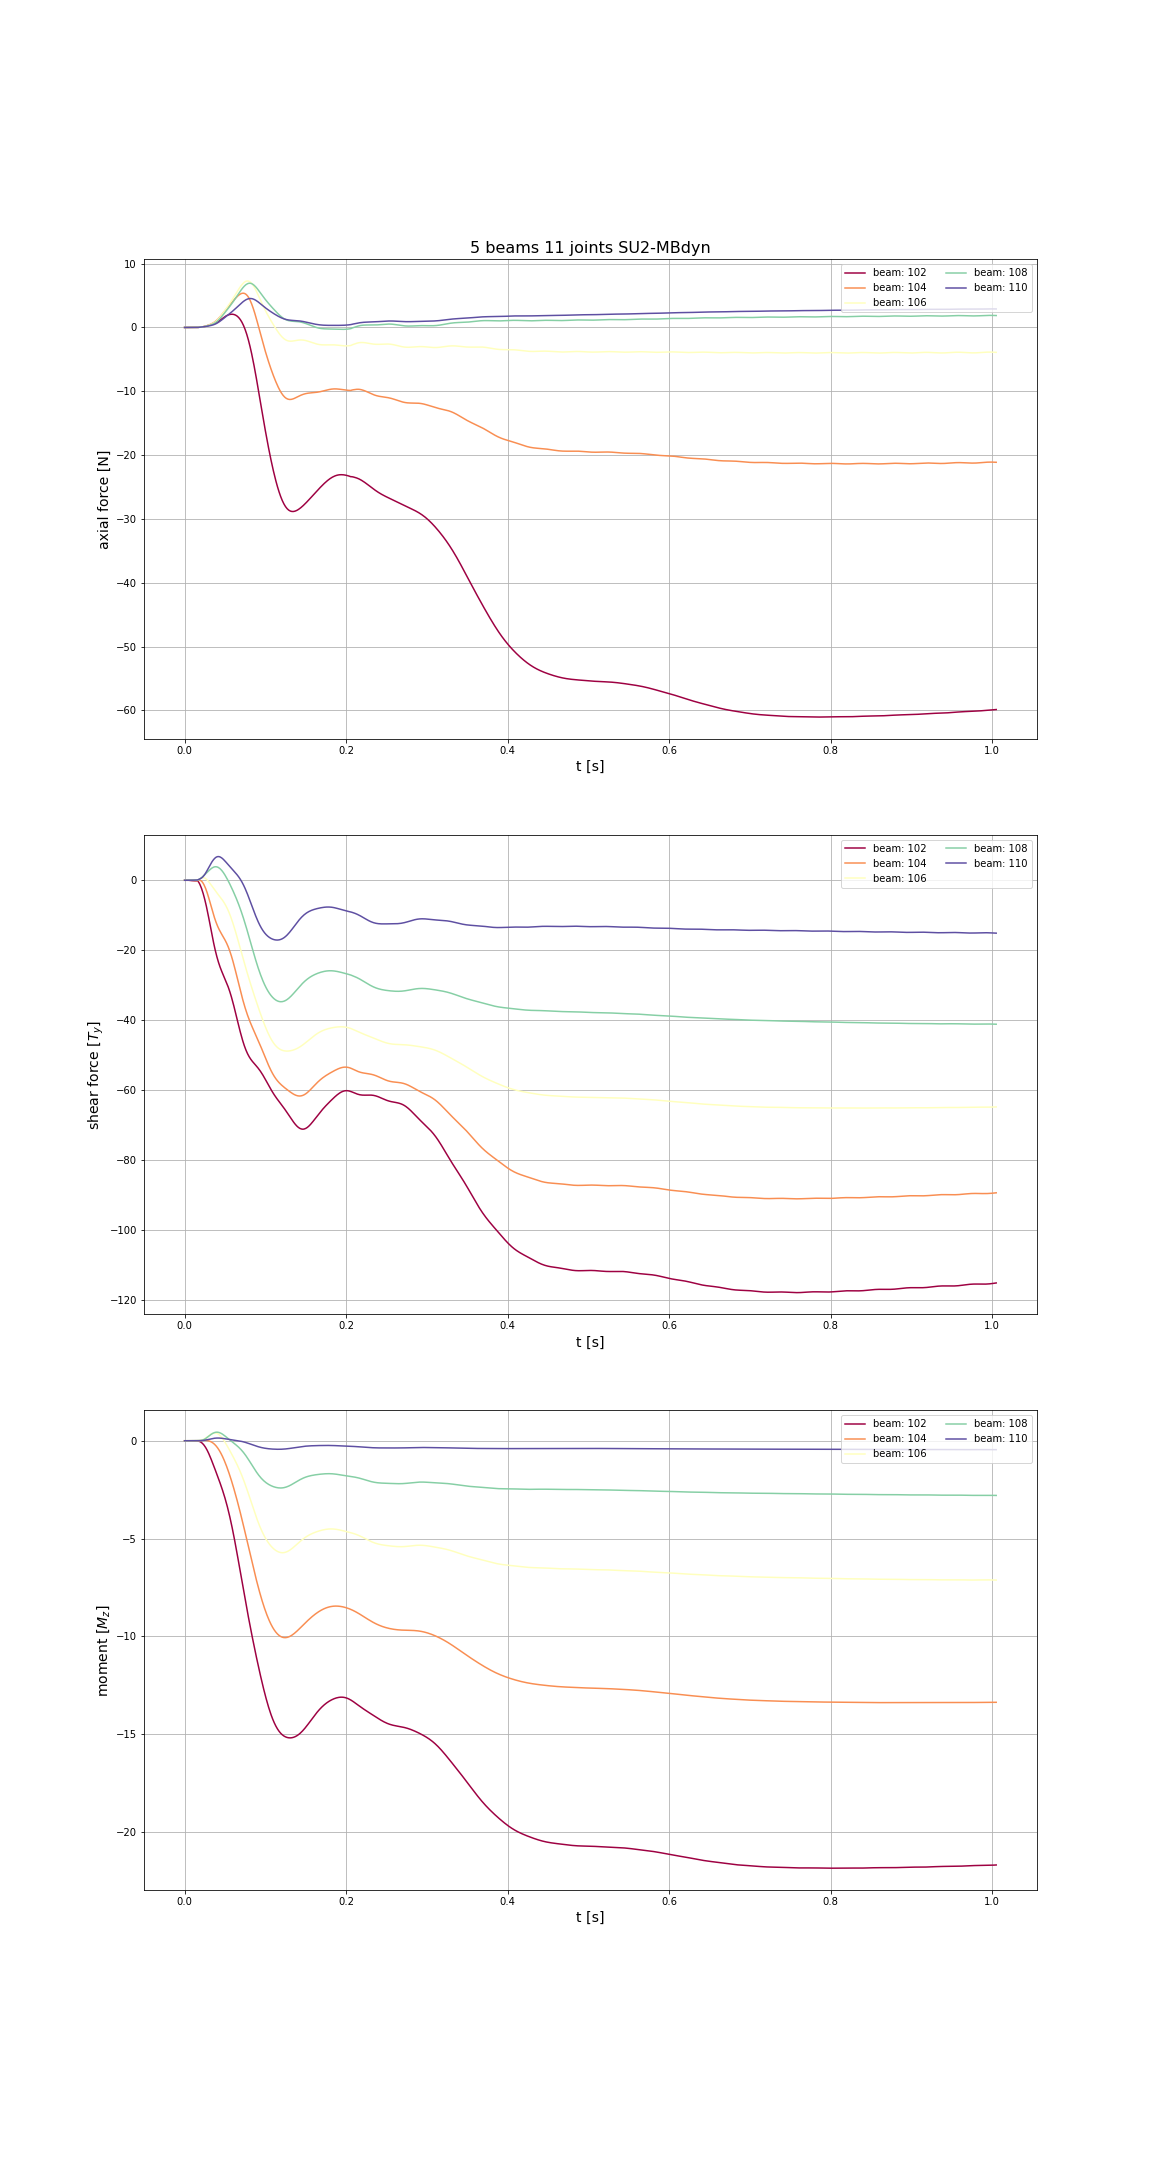
\includegraphics[width=0.92\textwidth, trim=0 230 0 230, clip]{images/comp_flap/vert-flap_SU2-MBDyn_act.png}
	\caption{vertical flap (compressible): MBDyn internal forces}
	\label{fig:comp_mbd_internal}
\end{figure}


\newpage


\section{Square bluff body Benchmark}
\label{sec:sq-cyl-bench}

The first simple problems aimed at verifying that the complete FSI problem: i.e. the MBDyn model, the mapping with the interface mesh, the coupling adapter and the fluid model (fluid flow and mesh movement performed with different solvers) is working and gives correct results.

After that it is important to verify the performance of the system considering well-known benchmarks, so that the results can be compared with a large number of algorithms and techniques.

\subsection{Problem description}

The first benchmark considered here has been described in \cite{ramm1998fluid}. The structural part is composed of a square bluff body with a trailing thin flap, as described in Figure \ref{fig:sq_domain}. The geometrical data are given in Table \ref{table:sq-geom}.

\begin{table}[!htb]
	\begin{center}
		\begin{tabular}{ l c | r } 
			parameter & & value   \\ 
			\hline
			H  & [\si{mm}] & $10$     \\
			L & [\si{mm}] & $40$  \\
			t  & [\si{mm}] & $0.6$  \\			
		\end{tabular}
	\end{center}
	\caption{square bluff body: geometry}
	\label{table:sq-geom}
\end{table}

\begin{figure}[htbp!]
	\centering
	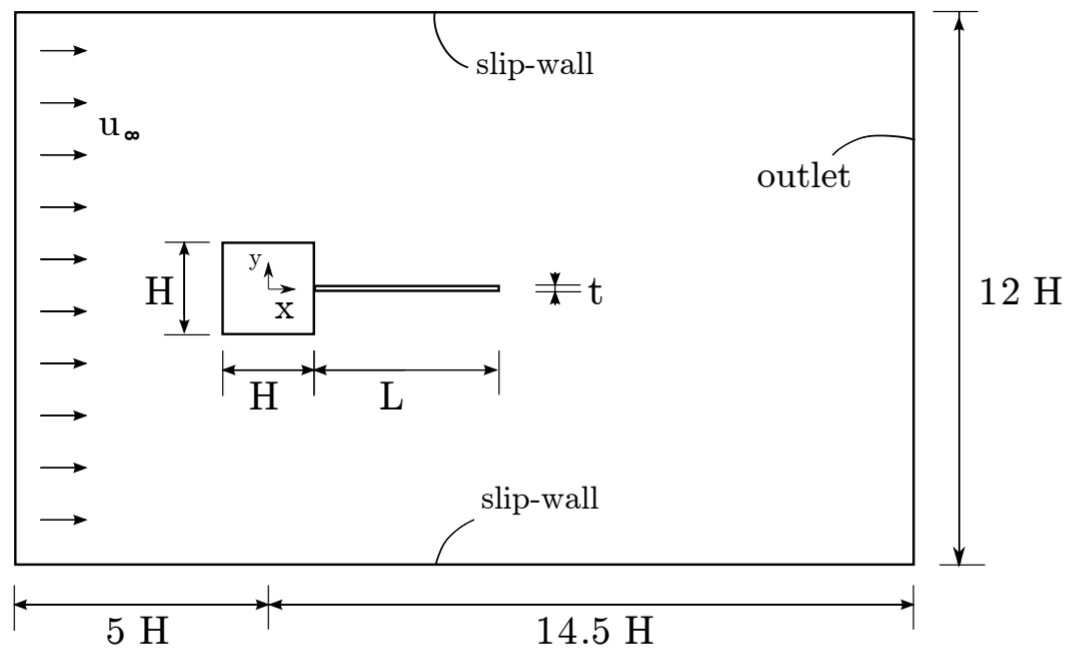
\includegraphics[width=0.82\textwidth, trim=0 0 0 0, clip]{images/sq-cyl/sq-cyl-domain.png}
	\caption{square bluff body benchmark: domain}
	\label{fig:sq_domain}
\end{figure}

\subsection{Fluid domain}

The fluid domain is represented in Figure \ref{fig:sq_domain} and has been simulated in OpenFOAM. The inlet is on the left with uniform flow velocity, the outlet is on the right, the external boundaries (top and bottom) are \textit{slip-walls} while all other boundaries (cylinder and flap) are \textit{no-slip} walls.


The fluid domain is discretized in an structured hexaedral mesh as depicted in Figure \ref{fig:sq_mesh}. The main fluid and mesh values are given in Table \ref{table:sq-fluid} and \ref{table:sq-mesh}. 

\begin{figure}[htbp!]
	\centering
	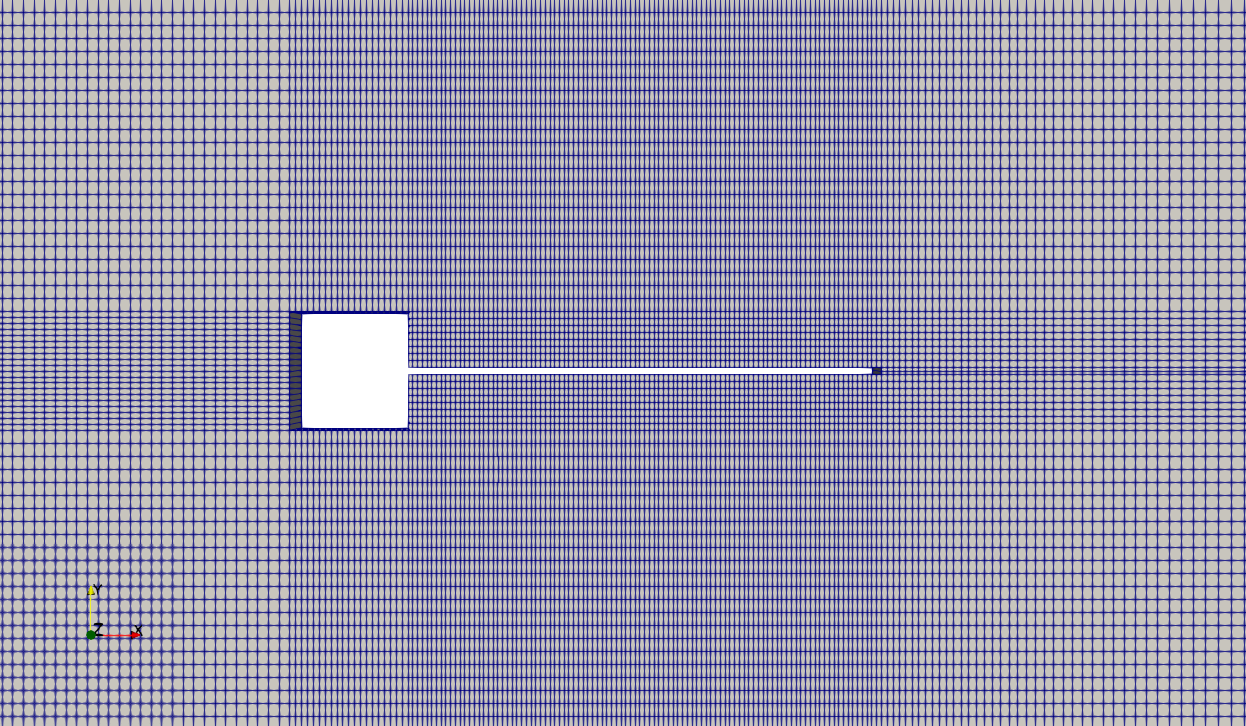
\includegraphics[width=0.9\textwidth]{images/sq-cyl/sq_mesh.png}
	\caption{square bluff body: fluid mesh}
	\label{fig:sq_mesh}
\end{figure}


\begin{table}[!htb]
	\begin{center}
		\begin{tabular}{ l c l | c } 
			parameter & & & value  \\ 
			\hline
			fluid density  & $\rho$ & \si{kg.m^{-3}} & $1.18$   \\
			dynamic viscosity & $\mu$& \si{kg.m^{-1}.s^{-1}} & $1.82 \cdot 10^{-5}$  \\
%			Reynolds length & $l_{Re}$ & $0.1$ & \si{m} \\
			Reynolds number & Re &  & $332$ \\
			flow velocity & $\vec{u}_{\infty}$ & \si{m.s^{-1}} & $0.513$ \\
			flow type & & & laminar \\
		\end{tabular}
	\end{center}
	\caption{square bluff body: fluid properties}
	\label{table:sq-fluid}
\end{table}



\begin{table}[!htb]
	\begin{center}
		\begin{tabular}{ l c | c } 
			parameter & & value   \\ 
			\hline
			number of mesh points  & $n_{dof}$ & 59096     \\
			number of cells & $n_c$ & 29040  \\
			number of interface cells  & $n_{int}$ & 202  \\			
		\end{tabular}
	\end{center}
	\caption{square bluff body: mesh properties}
	\label{table:sq-mesh}
\end{table}


\subsection{Solid domain}

The properties of the solid are reported in Table \ref{table:sq-solid}.

\begin{table}[!htb]
	\begin{center}
		\begin{tabular}{ l c  l | c } 
			parameter & & value &    \\ 
			\hline
			solid density  & $\rho$ & \si{kg.m^{-3}} & 100    \\
			Elastic modulus  & E & \si{Pa} & $2.5\cdot 10^5$    \\
			Poisson coefficient & $\nu$ & & $0.35$  \\
			%			Reynolds length & $l_{Re}$ & $0.1$ & \si{m} \\
			%			Reynolds number & Re & $\approx 1000$ & \\
		\end{tabular}
	\end{center}
	\caption{square bluff body: solid properties}
	\label{table:sq-solid}
\end{table}

The MBDyn model is composed of 10 \texttt{beam3} elements. The setup resembles the one briefly described in Section \ref{sec:dummy}. The structural damping of the beam elements (see Section \ref{sec:mbd-beam}) has been set to be proportional to stiffness matrix of the element with a coefficient of $1\cdot10^{-2}$. This value appeared to be high enough to give a smooth structural solution without being excessively damping.

The interface mesh is divided into 202 faces and is shown in Figure \ref{fig:sq_struct_mesh}. 

\begin{figure}[htbp!]
	\centering
	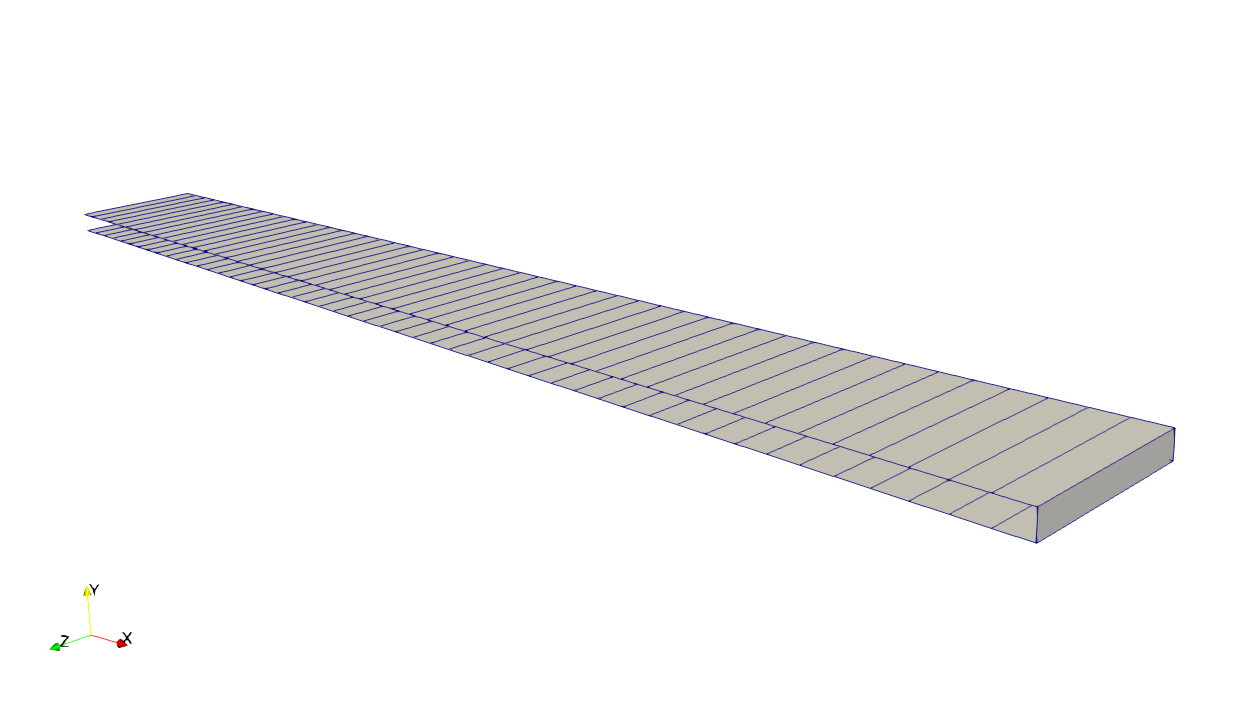
\includegraphics[width=0.9\textwidth, trim=0 50 0 200, clip]{images/sq-cyl/sq_struct_mesh.png}
	\caption{square bluff body: structural interface mesh}
	\label{fig:sq_struct_mesh}
\end{figure}


\subsection{Coupling parameters}


The main coupling data are given in Table \ref{table:sq-coupling}. The particularly short time step is required by fluid mesh movement: as it will be apparent in the results, the thin flexible flap moves quickly and with large displacement. The diffusion algorithm used by OpenFOAM to deform the fluid mesh produced inconsistent cell volumes when using higher time steps. 

\begin{table}[!htb]
	\begin{center}
		\begin{tabular}{ l c  l| c } 
			parameter & & & value   \\ 
			\hline
			simulation time  & $t$& \si{s} & 6      \\
			step size & $\Delta t$ & \si{s} & $5 \cdot 10^{-4}$   \\
			\hline
			coupling scheme & & & serial implicit  $S\rightarrow F$  \\
			coupling algorithm & & &  IQN-ILS  \\
			displacement rel. convergence limit & & & $10^{-4}$ \\
			force rel. convergence limit &&  & $10^{-3}$  \\
      		interface mesh mapping & & & RBF  \\
			
		\end{tabular}
	\end{center}
	\caption{square bluff body: coupling parameters}
	\label{table:sq-coupling}
\end{table}

Most parameters are similar to the ones used in other examples as they turned out to fit well with most of the experiments. 

\subsection{Results}

The problem considered is characterized by the adimensional parameters given in Table \ref{table:sq-adim} and its solution is represented in Figure \ref{fig:sq_sol}.

\begin{table}[!htb]
	\begin{center}
		\begin{tabular}{ l c | r } 
			parameter & & value   \\ 
			\hline
			mass number  & $M$ & $ 1.18\cdot 10^{-2}$     \\
			reduced velocity & $U_R$ & $ \approx 1\cdot 10^{-2}$  \\
			Cauchy number  & $C_Y$ & $  1.24 \cdot 10^{-6}$  \\			
		\end{tabular}
	\end{center}
	\caption{square bluff body: adimensional numbers}
	\label{table:sq-adim}
\end{table}

As in other simulations, fluid forces are applied with a ramp to ease convergence at the beginning of the simulation: during the first $100$ \si{ms} they are scaled to $10\%$ to reach $100\%$ after another $100$ \si{ms}.

Alternating vortices begin developing quite rapidly and the structure begins oscillating. After around 2 seconds reaches a vortex lock-in regime (e.g. \cite{hong2001fluid}), as shown in Figure \ref{fig:sq_displacement} (in particular the tip displacement in \textit{y} direction).



\begin{figure}[htbp!]
	\centering
	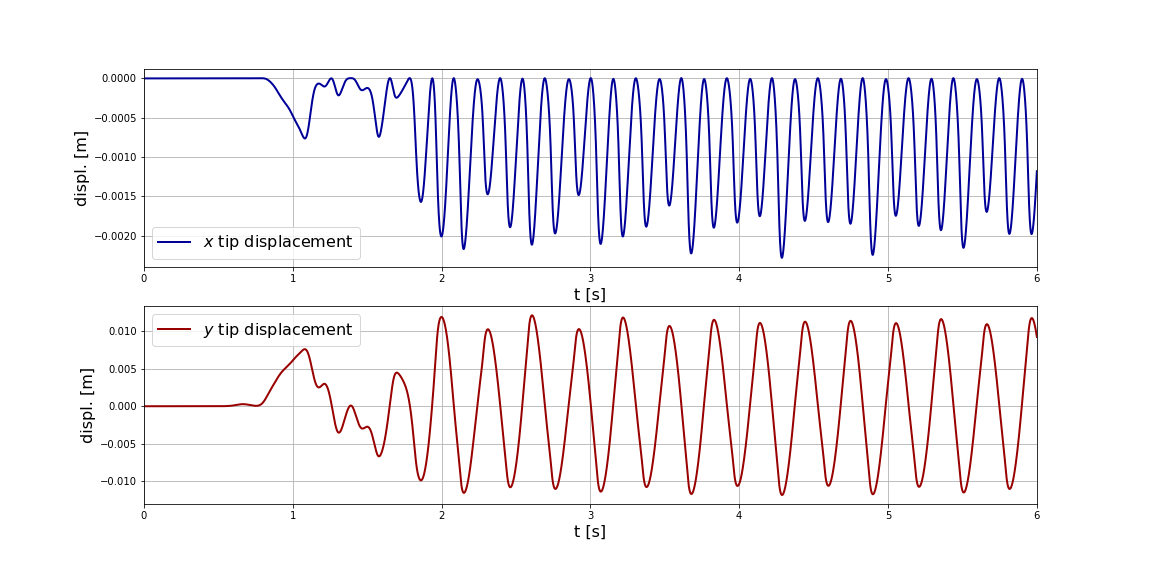
\includegraphics[width=0.98\textwidth, trim=20 20 20 50, clip]{images/sq-cyl/disp_sq.png}
	\caption{square bluff body: tip displacement}
	\label{fig:sq_displacement}
\end{figure}

Forces are measured on the whole structure on the fluid side, while are measured on the flap in the solid domain. Figure \ref{fig:sq_force} shows a detail of $0.5$ \si{s} of simulation. The difference in \textit{x}-direction represents the drag force on the cylinder. Differences in lift and moment are almost zero. 

\begin{figure}[htbp!]
	\centering
	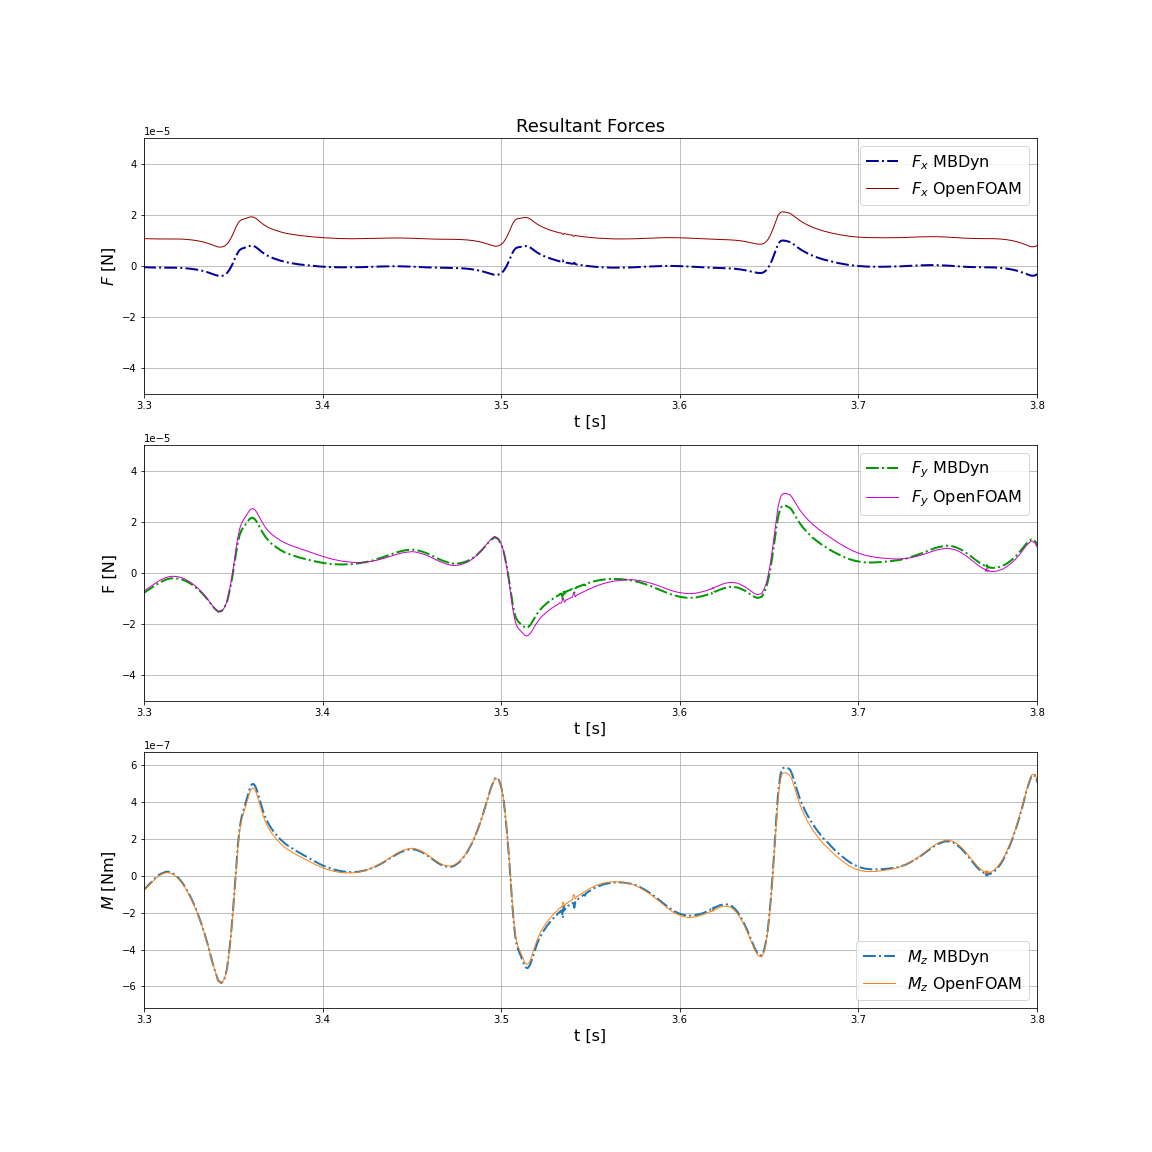
\includegraphics[width=0.98\textwidth, trim=20 100 20 100, clip]{images/sq-cyl/forces_sq.png}
	\caption{square bluff body: resultant forces (detail)}
	\label{fig:sq_force}
\end{figure}


\begin{figure}[htb]
\centering % <-- added
\begin{subfigure}{0.5\textwidth}
  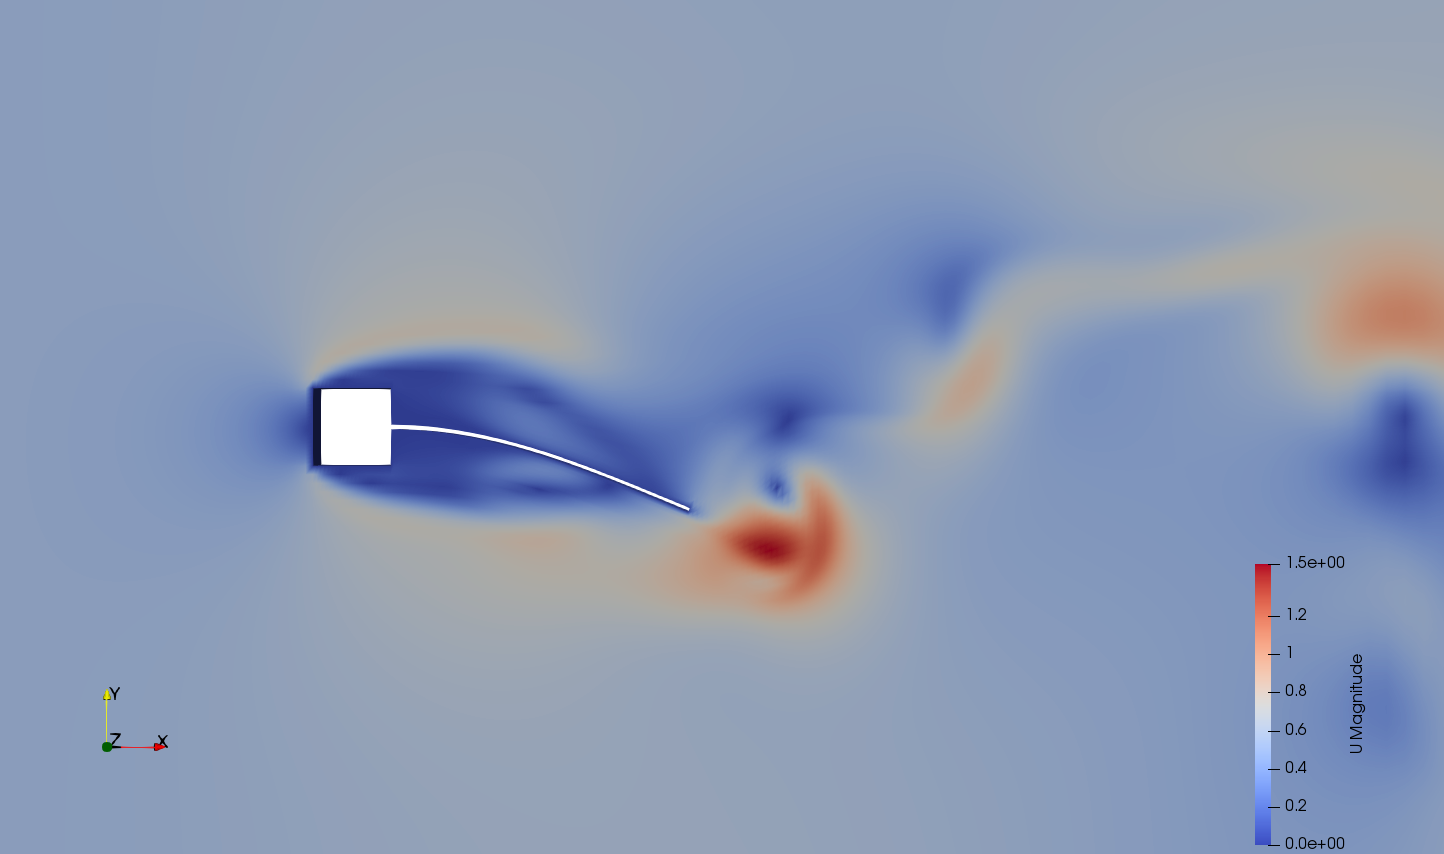
\includegraphics[width=\linewidth]{images/sq-cyl/sq_v1.png}
  \caption{t=3.37s velocity}
  \label{fig:sq_v1}
\end{subfigure}\hfil % <-- added
\begin{subfigure}{0.5\textwidth}
  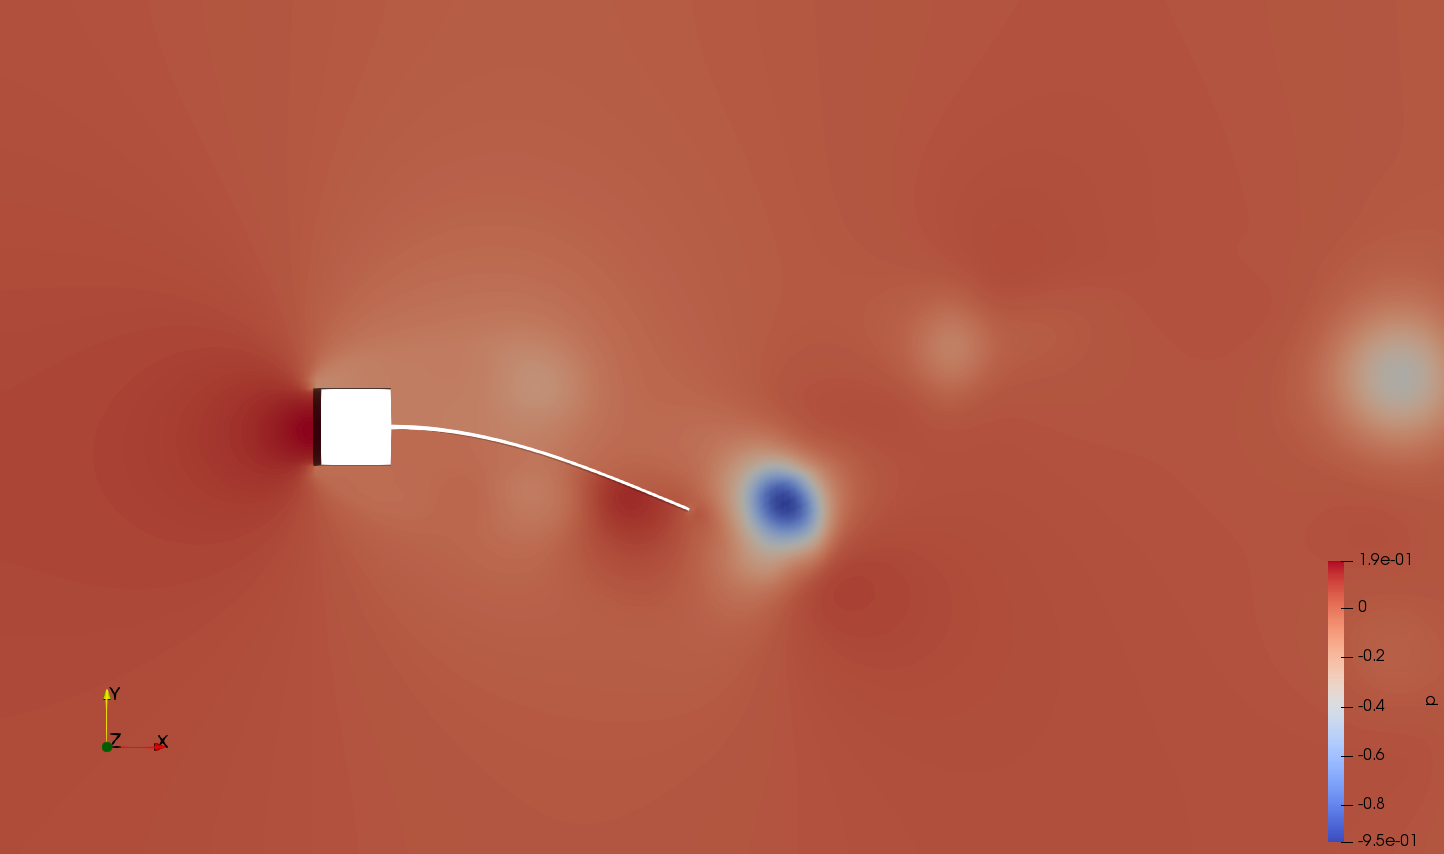
\includegraphics[width=\linewidth]{images/sq-cyl/sq_p1.png}
  \caption{t=3.37s pressure}
  \label{fig:sq_p1}
\end{subfigure}\hfil % <-- added

\medskip

\begin{subfigure}{0.5\textwidth}
  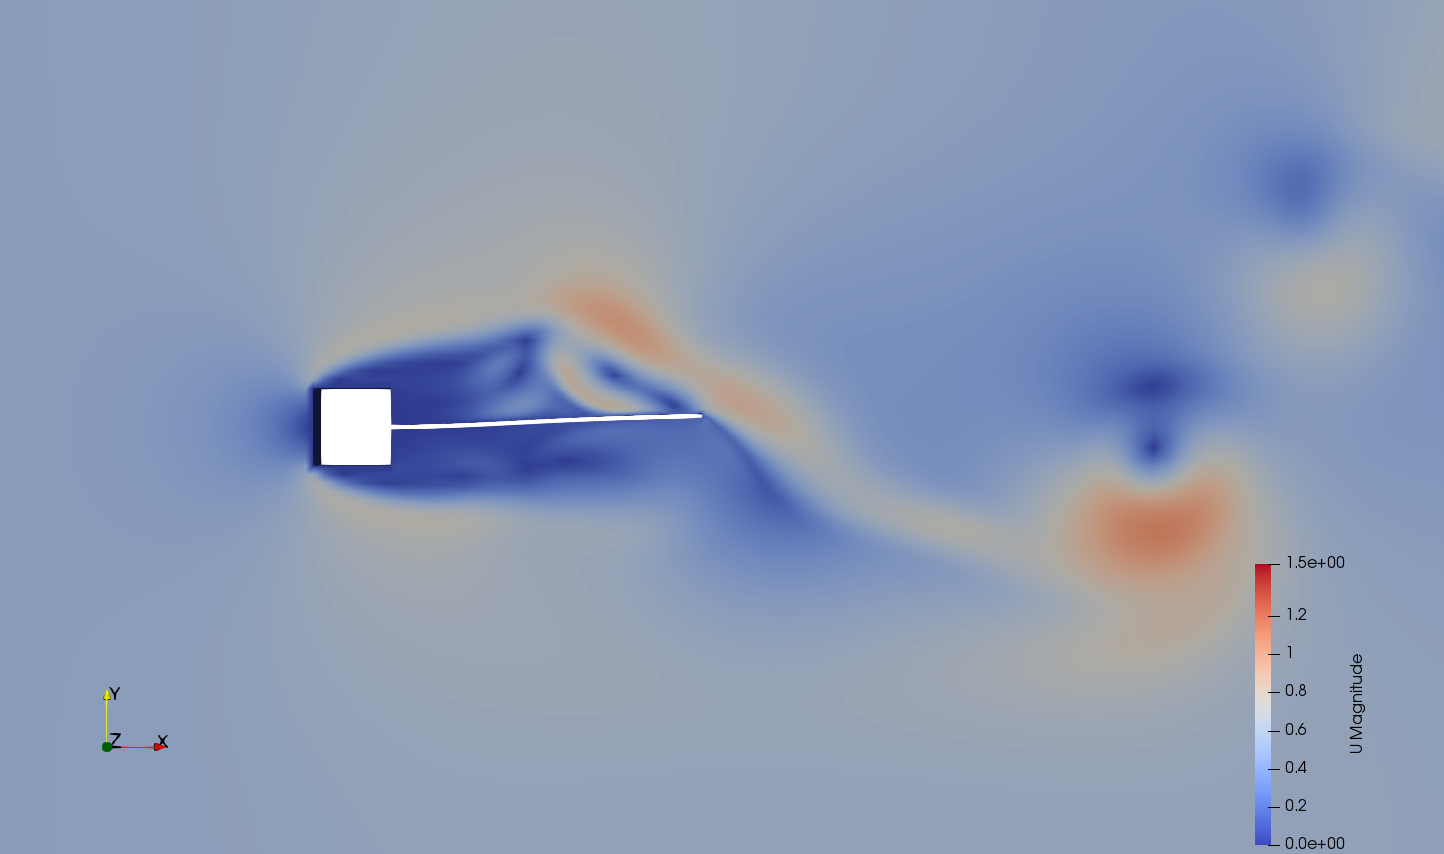
\includegraphics[width=\linewidth]{images/sq-cyl/sq_v2.png}
  \caption{t=3.47s velocity}
  \label{fig:sq_v2}
\end{subfigure}\hfil % <-- added
\begin{subfigure}{0.5\textwidth}
  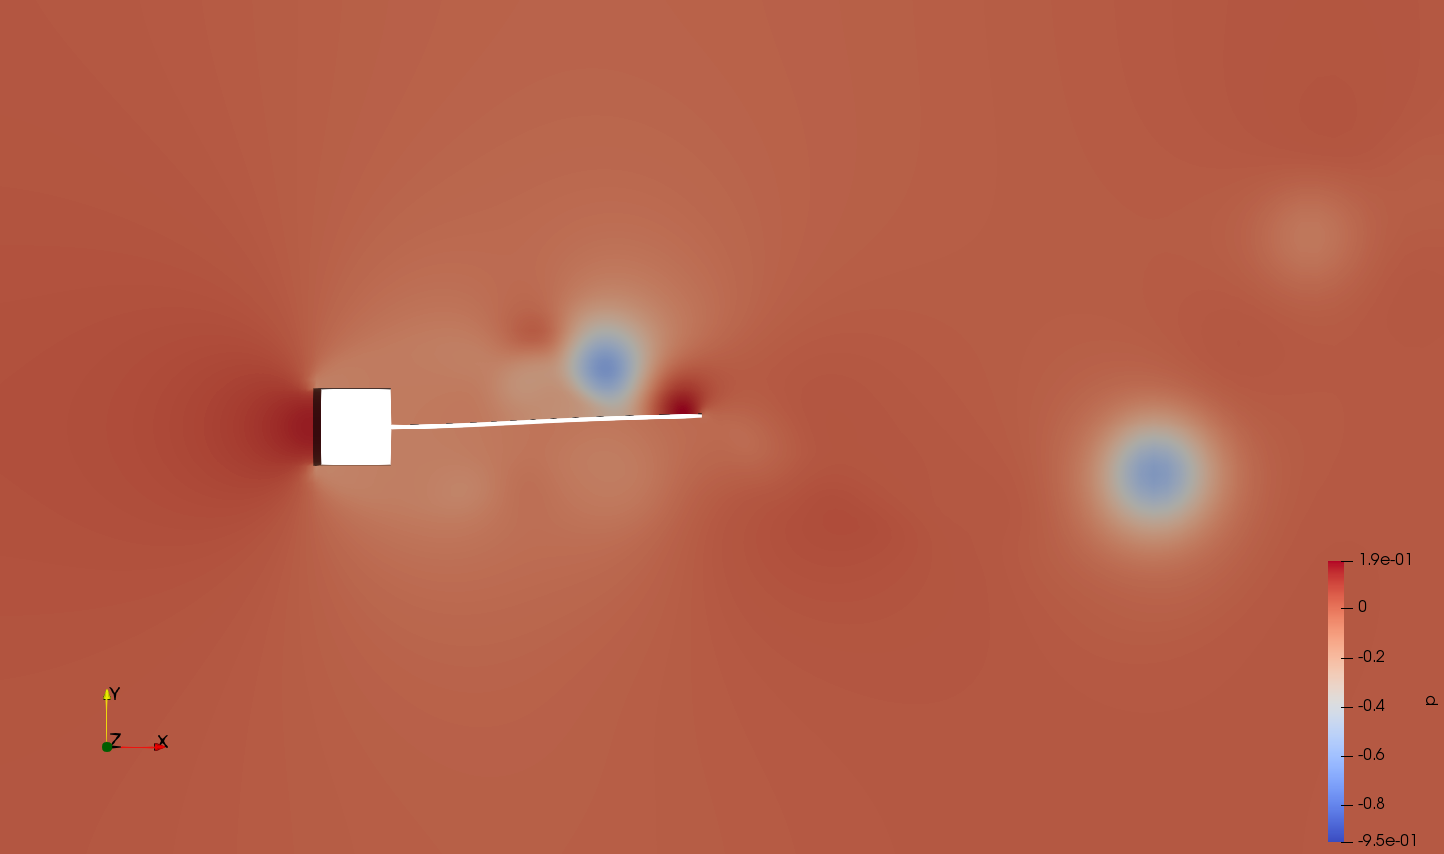
\includegraphics[width=\linewidth]{images/sq-cyl/sq_p2.png}
  \caption{t=3.47s pressure}
  \label{fig:sq_p2}
\end{subfigure}\hfil % <-- added

\medskip

\begin{subfigure}{0.5\textwidth}
  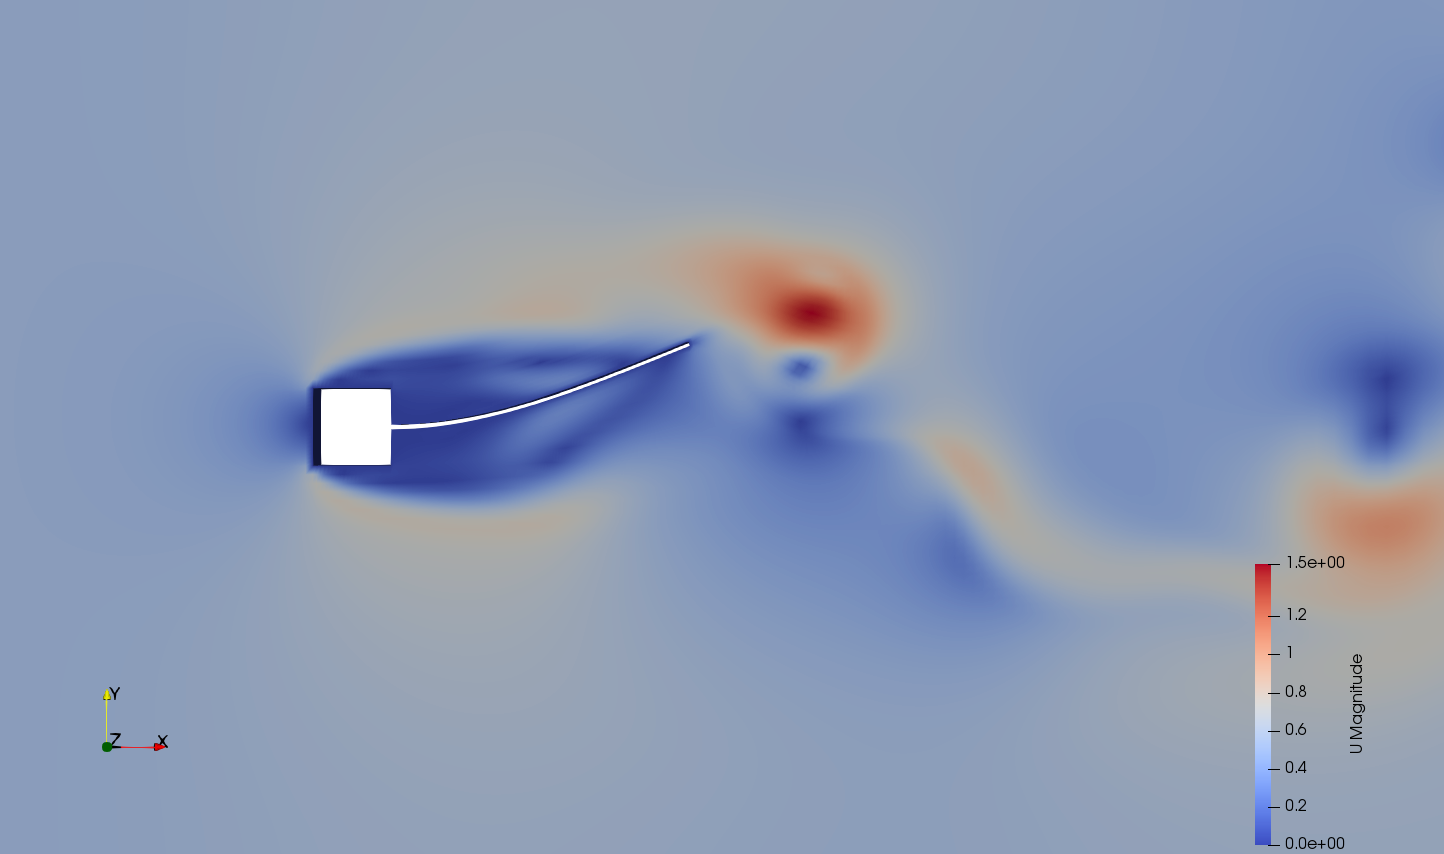
\includegraphics[width=\linewidth]{images/sq-cyl/sq_v3.png}
  \caption{t=3.53s velocity}
  \label{fig:sq_v3}
\end{subfigure}\hfil % <-- added
\begin{subfigure}{0.5\textwidth}
  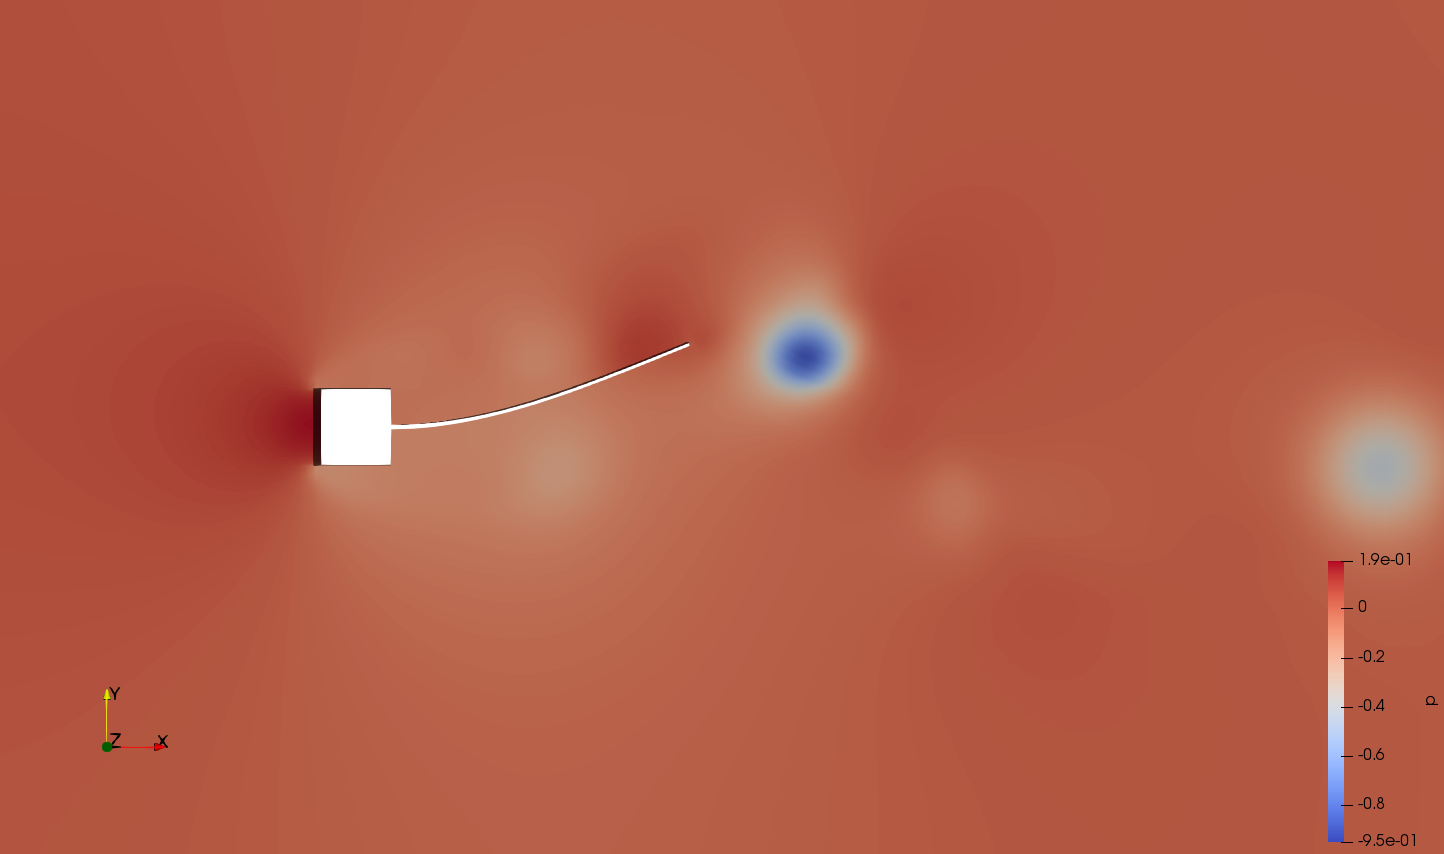
\includegraphics[width=\linewidth]{images/sq-cyl/sq_p3.png}
  \caption{t=3.53s pressure}
  \label{fig:sq_p3}
\end{subfigure}\hfil % <-- added

\caption{square bluff body: fluid solution}
\label{fig:sq_sol}
\end{figure}


Each time step converges with an average of 8 iterations, except for some situations where the coupling algorithm fails in making coupling forces converge. Those situations show a quite distorted fluid mesh that make the overall FSI problem harder to solve.

An higher average number of iterations agrees with the fact that a higher mass number, here in the order of $\mathcal{O} \left(10^{-2} \right) $, makes the problem strongly coupled.

\begin{figure}[htbp!]
	\centering
	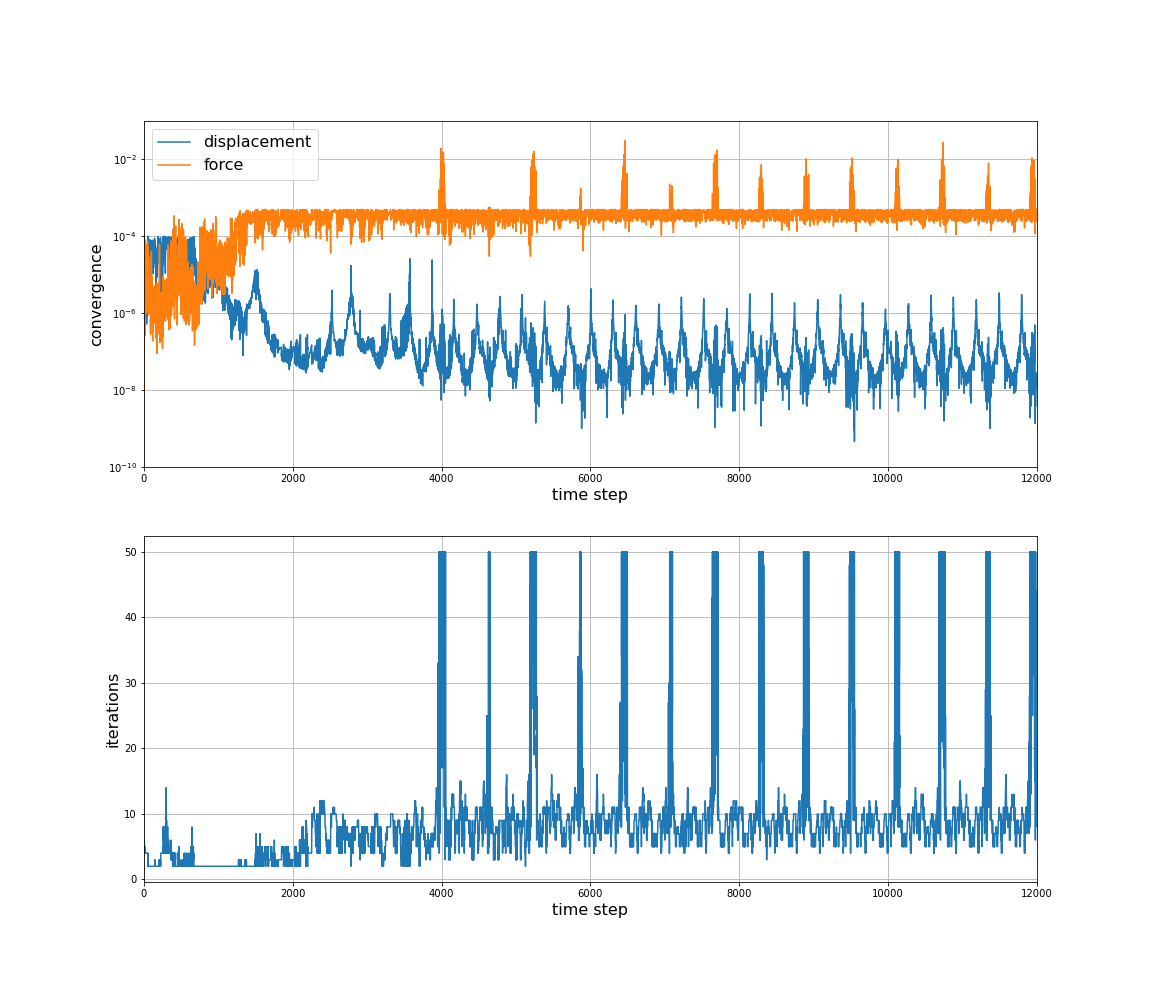
\includegraphics[width=0.95\textwidth, trim=0 80 0 100, clip]{images/sq-cyl/MBD_iterations_sq.png}
	\caption{square bluff body: convergence and iterations}
	\label{fig:sq_mbd_iter}
\end{figure}

As in the previous examples, the axial, shear and bending moment in each of the MBDyn elements are plotted in Figure \ref{fig:sq_mbd_internal}: in this case a temporal slice of $0.5s$ has been considered.

\begin{figure}[htbp!]
	\centering
	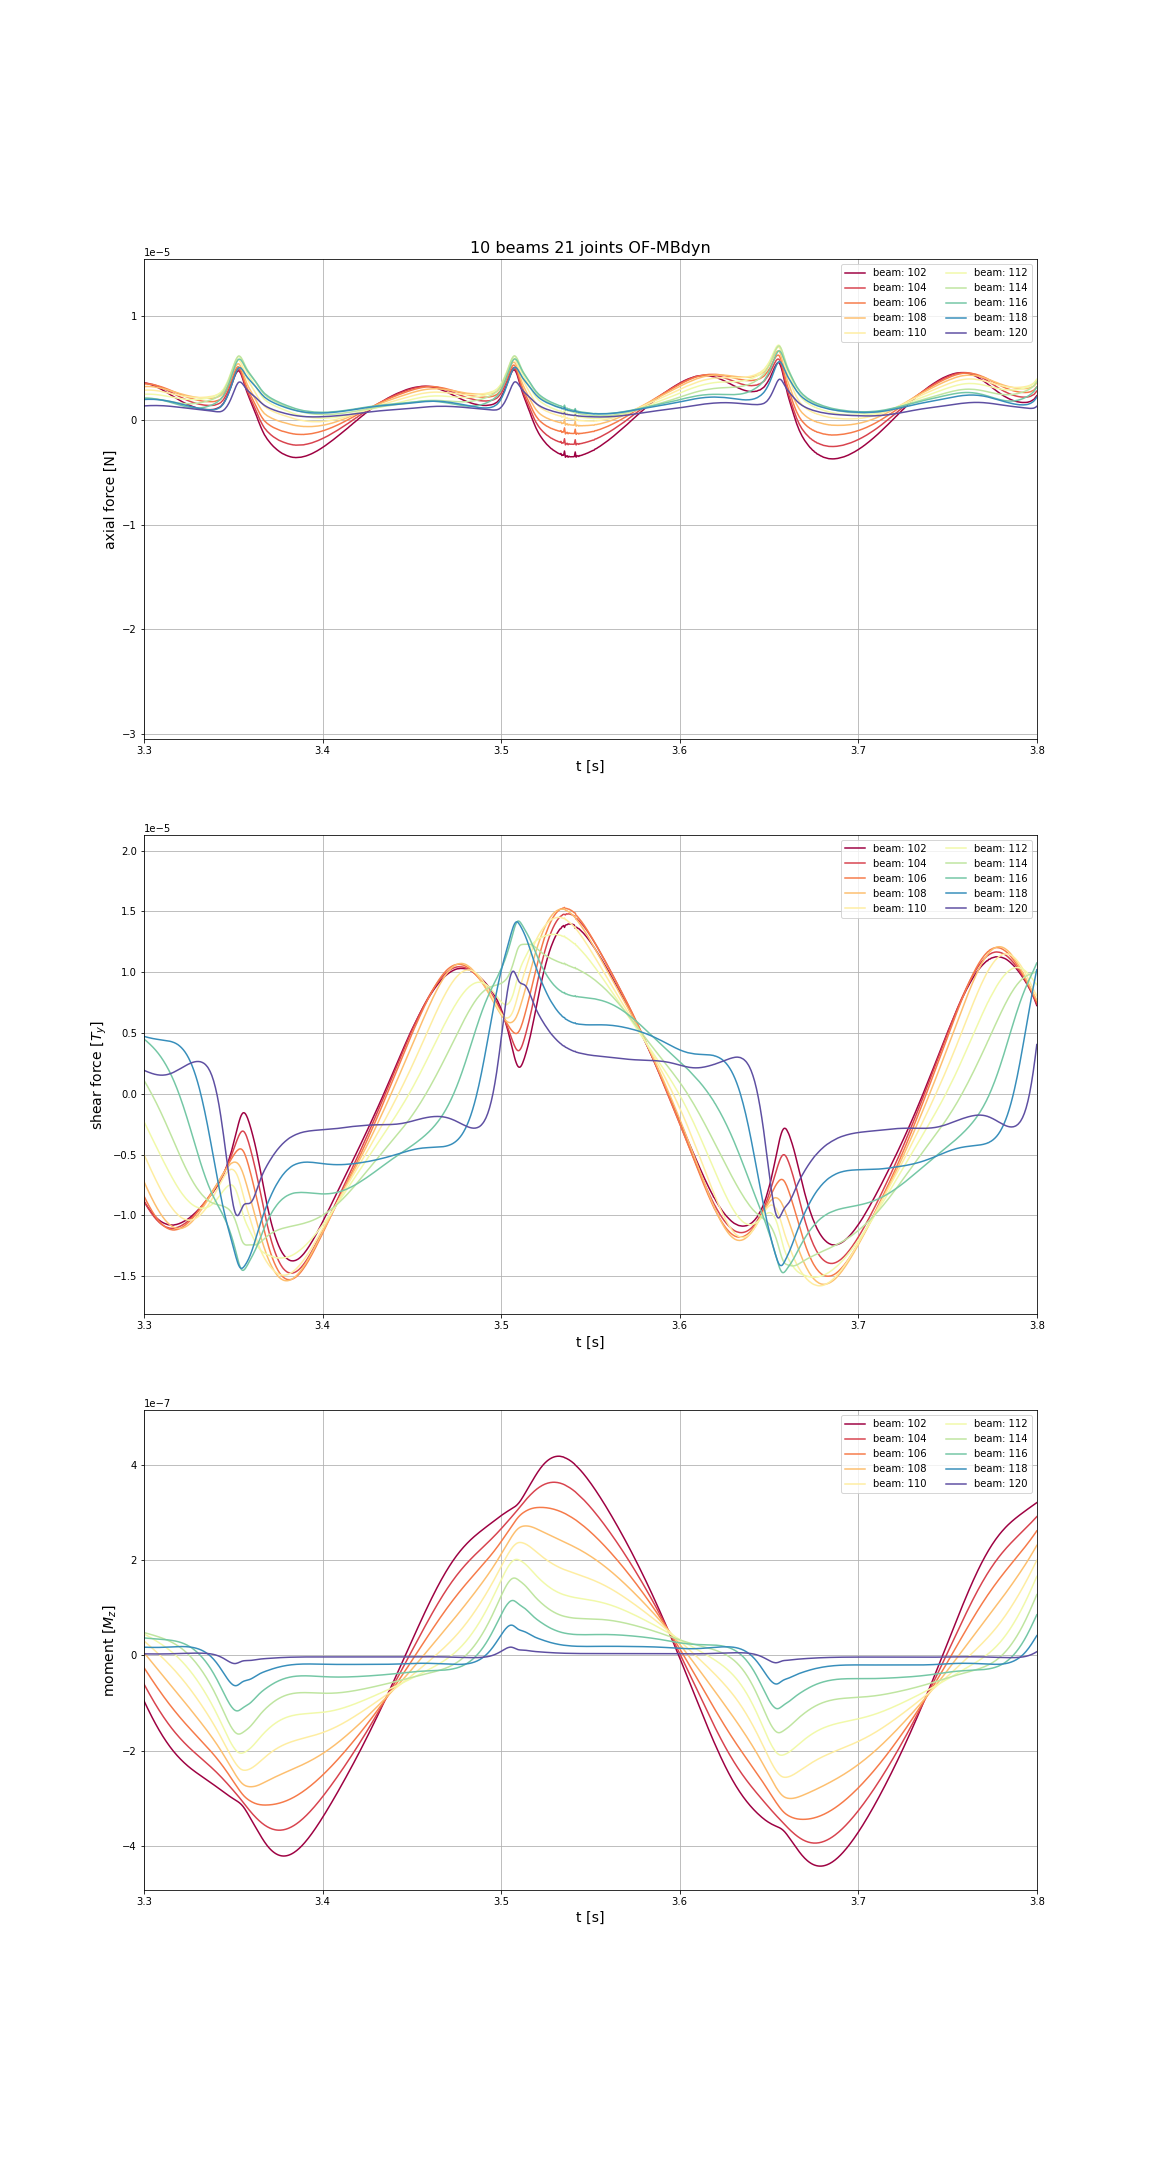
\includegraphics[width=0.92\textwidth, trim=0 230 0 230, clip]{images/sq-cyl/sq-flap_OF-MBDyn_act.png}
	\caption{square bluff body: MBDyn internal forces (detail)}
	\label{fig:sq_mbd_internal}
\end{figure}

\newpage

\subsection{Validation}

This problem has been used as a benchmark in a great number of studies in literature. The comparison between the studies is generally made on the tip displacement, in term of amplitude and frequency of oscillation. In Table \ref{table:sq-res} some results are given and compared to the present study.

\begin{table}[!ht]
	\begin{center}
		\begin{tabular}{ l | c  c } 
			Study & $f$ [\si{s^{-1}}] & $d_{y tip}$ [\si{mm}]   \\ 
			\hline
            Wall and Ramm \cite{ramm1998fluid} & $3.08$ & $13.1$ \\
            Kassiotis et al. \cite{kassiotis2011nonlinear} & $2.98$ & $10.5$ \\
            Wood et al. \cite{wood2010partitioned} & $2.94$ & $11.5$ \\
            Olivier et al. \cite{olivier2009fluid} & $3.17$ & $9.5$ \\
            Walhorn et al. \cite{walhorn2002space} & $3.14$ & $10.2$ \\
            Matthies and Steindorf \cite{matthies2003partitioned} & $3.13$ & $11.8$ \\ 
            Dettmer and Peric \cite{dettmer2006computational} & $3.03$ & $12.5$ \\
            Habchi et al. \cite{habchi2013partitioned} & $3.25$ & $10.2$ \\
            Froehle and Persson \cite{froehle2014high} & $3.18$ & $11.2$ \\
            Sanchez et al.\tablefootnote{Fluid Structure Interaction Problems using SU2. First SU2 Annual Developers Meeting. TU Delft, 6 September 2016}  & $3.15$ & $11.5$ \\
            \hline
            Present study    & $3.067$ & $11.2$ \\
            
		\end{tabular}
	\end{center}
	\caption{square bluff body: results}
	\label{table:sq-res}
\end{table}

The comparison shows a very good agreement among the studies: considering all the previous simulations, the average tip displacement is $11.2$ \si{mm} with a standard deviation of $1.06$ \si{mm} and the average frequency of oscillation is $3.1$ \si{Hz} with a standard deviation of $0.09$ \si{Hz}. 
This study, with a tip displacement of $11.2$ \si{mm} at a frequency of $3.067$ \si{Hz}, shows that the implementation of the adapter can give good results.

\newpage

\section{Turek-Hron FSI2 Benchmark}
\label{sec:FSI2}


Another well known benchmark concerning FSI simulations performed in incompressible flow regime is proposed by Turek and Hron \cite{turek2006proposal}.
A very important thing to notice about this study is that it is a proposal for a benchmark, as it is called  ``Proposal for numerical benchmarking of fluid-structure interaction between an elastic object and laminar incompressible flow''. So the paper gives a specific problem setup which others can contribute.

The fluid domain is similar to the one described in the previous chapter. The domain is again composed by a cylinder and a flap, but different flow velocities and structural properties are considered, so that 3 cases arise, commonly knonw as FSI1, FSI2 and FSI3.

For reasons that will be apparent in the next section, FSI2 is considered first. 

\subsection{Problem Description}

The structural part is composed of a round cylinder with a trailing thin flap, as described in Figure \ref{fig:fsi2_domain}. The geometrical data are given in Table \ref{table:fsi2-geom}.

\begin{table}[!htb]
	\begin{center}
		\begin{tabular}{ l c | r } 
			parameter & & value   \\ 
			\hline
			H  & [\si{m}] & $0.41$     \\
			L &  [\si{m}] & $2.5$  \\
			l  & [\si{m}] & $0.35$  \\
			h  & [\si{m}] & $0.02$  \\
			C  & [\si{m}] & $\left(0.2,0.2 \right)$  \\
			r  & [\si{m}] & $0.05$  \\
		\end{tabular}
	\end{center}
	\caption{FSI2: geometry}
	\label{table:fsi2-geom}
\end{table}

\begin{figure}[htbp!]
	\centering
	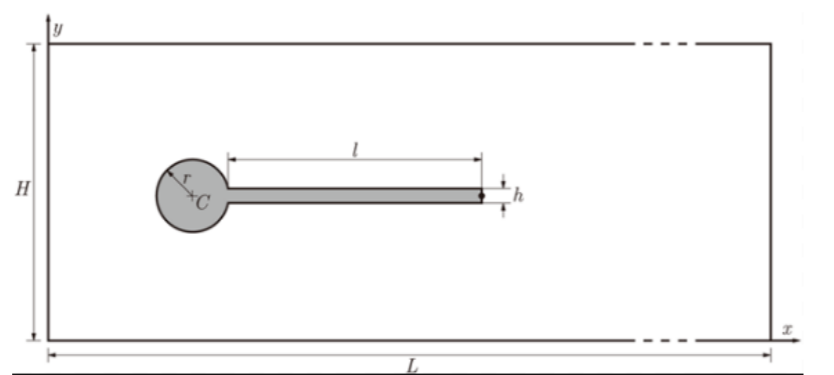
\includegraphics[width=0.92\textwidth, trim=0 0 50 0, clip]{images/FSI2/FSI2.png}
	\caption{FSI2: domain}
	\label{fig:fsi2_domain}
\end{figure}

\subsection{Fluid domain}

The fluid domain is represented in Figure \ref{fig:fsi2_domain} and has been simulated in OpenFOAM. The inlet is on the left with \textit{parabolic} flow velocity, the outlet is on the right, while all other boundaries are \textit{no-slip} walls.

The fluid domain is discretized in an structured hexaedral mesh as depicted in Figure \ref{fig:FSI2_mesh}. The main fluid and mesh values are given in Table \ref{table:FSI2-fluid} and \ref{table:FSI2-mesh}. 

\begin{figure}[htbp!]
	\centering
	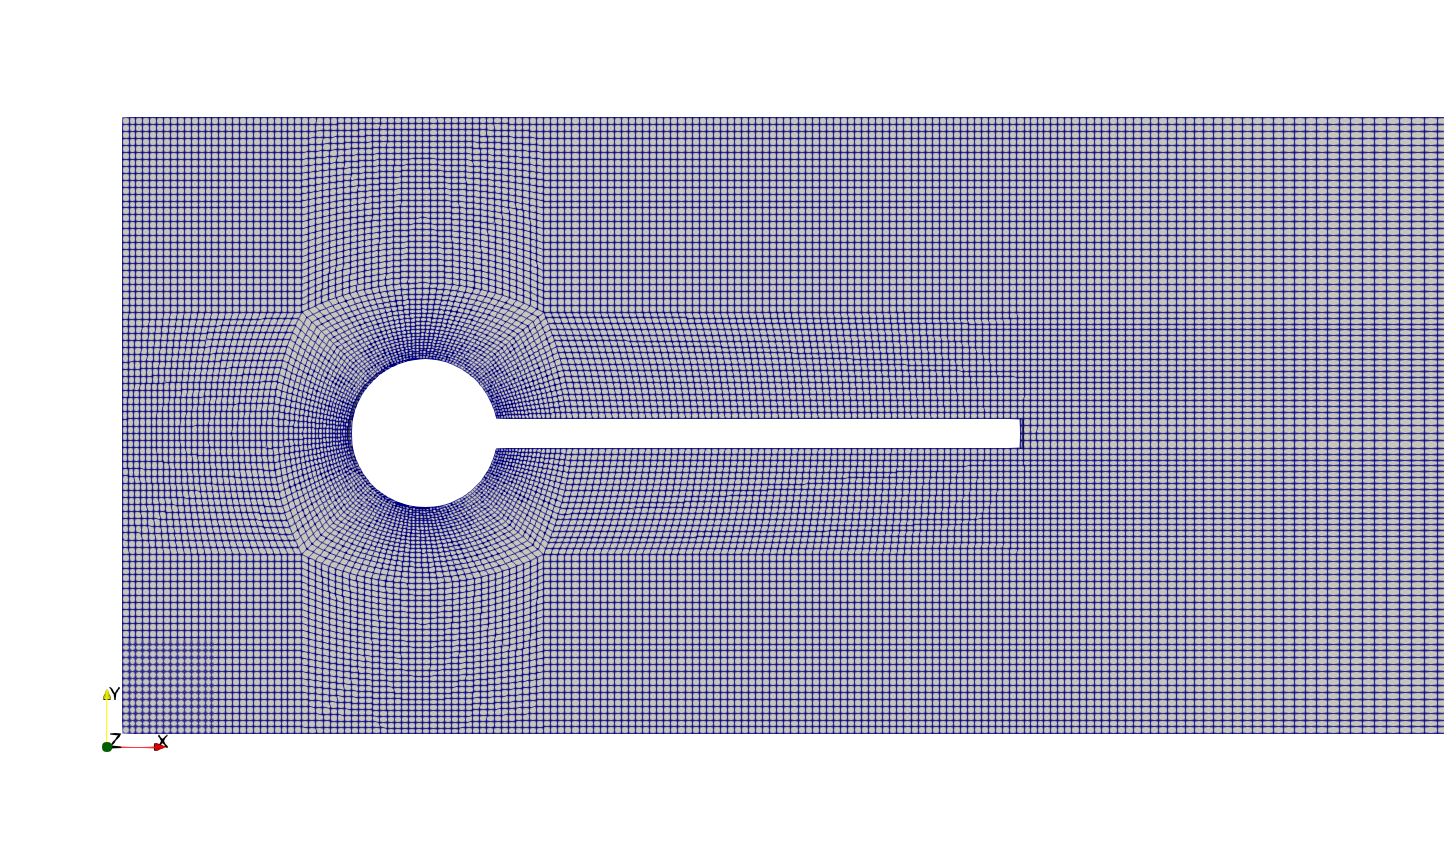
\includegraphics[width=0.9\textwidth]{images/FSI2/FSI2-mesh.png}
	\caption{FSI2: fluid mesh}
	\label{fig:FSI2_mesh}
\end{figure}


\begin{table}[!htb]
	\begin{center}
		\begin{tabular}{ l c l | c } 
			parameter & & & value  \\ 
			\hline
			fluid density  & $\rho$ & \si{kg.m^{-3}} & $1000$   \\
			kinematic viscosity & $\nu$& \si{m^{2}.s^{-1}} & $1 \cdot 10^{-3}$  \\
%			Reynolds length & $l_{Re}$ & $0.1$ & \si{m} \\
			Reynolds number & Re &  & $100$ \\
			max flow velocity & $\vec{u}_{max}$ & \si{m.s^{-1}} & $1.5$ \\
			mean flow velocity & $\vec{u}$ & \si{m.s^{-1}} & $1$ \\
			flow type & & & laminar \\
		\end{tabular}
	\end{center}
	\caption{FSI2: fluid properties}
	\label{table:FSI2-fluid}
\end{table}



\begin{table}[!htb]
	\begin{center}
		\begin{tabular}{ l c | c } 
			parameter & & value   \\ 
			\hline
			number of mesh points  & $n_{dof}$ & 51464     \\
			number of cells & $n_c$ & 25224  \\
			number of interface cells  & $n_{int}$ & 180  \\			
		\end{tabular}
	\end{center}
	\caption{FSI2: mesh properties}
	\label{table:FSI2-mesh}
\end{table}


\subsection{Solid domain}

The properties of the solid are reported in Table \ref{table:FSI2-solid}.

\begin{table}[!htb]
	\begin{center}
		\begin{tabular}{ l c  l | c } 
			parameter & & value &    \\ 
			\hline
			solid density  & $\rho$ & \si{kg.m^{-3}} & $10000$    \\
			Elastic modulus  & E & \si{Pa} & $1.4\cdot 10^6$    \\
			Poisson coefficient & $\nu$ & & $0.4$  \\
			%			Reynolds length & $l_{Re}$ & $0.1$ & \si{m} \\
			%			Reynolds number & Re & $\approx 1000$ & \\
		\end{tabular}
	\end{center}
	\caption{FSI2: solid properties}
	\label{table:FSI2-solid}
\end{table}

The MBDyn model is the same as the one used in \ref{sec:sq-cyl-bench} and is composed of 10 \texttt{beam3} elements, with a structural damping of $1\cdot10^{-2}$.

The interface mesh is divided into 90 faces and is shown in Figure \ref{fig:FSI2_struct_mesh}. 

\begin{figure}[htbp!]
	\centering
	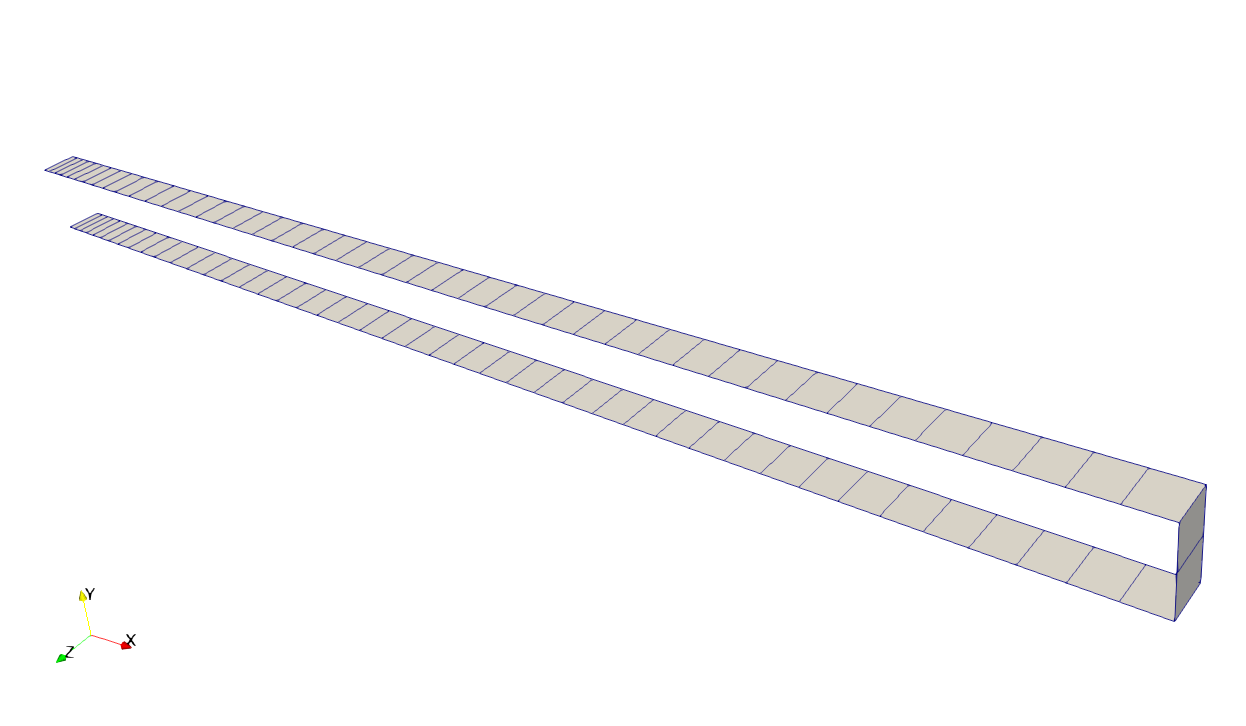
\includegraphics[width=0.9\textwidth, trim=0 50 0 150, clip]{images/FSI2/fsi2_struct_mesh.png}
	\caption{FSI2: structural interface mesh}
	\label{fig:FSI2_struct_mesh}
\end{figure}


\subsection{Coupling parameters}


The main coupling data are given in Table \ref{table:FSI2-coupling}. In this case a time step of $1ms$ is enough for the simulation.

\begin{table}[!htb]
	\begin{center}
		\begin{tabular}{ l c  l| c } 
			parameter & & & value   \\ 
			\hline
			simulation time  & $t$& \si{s} & 15      \\
			step size & $\Delta t$ & \si{s} & $1 \cdot 10^{-3}$   \\
			\hline
			coupling scheme & & & serial implicit  $S\rightarrow F$  \\
			coupling algorithm & & &  IQN-ILS  \\
			displacement rel. convergence limit & & & $10^{-4}$ \\
			force rel. convergence limit &&  & $2 \cdot 10^{-4}$  \\
      		interface mesh mapping & & & RBF  \\
			
		\end{tabular}
	\end{center}
	\caption{FSI2: coupling parameters}
	\label{table:FSI2-coupling}
\end{table}


\subsection{Results}

The problem considered is characterized by the adimensional parameters given in Table \ref{table:FSI2-adim} and its solution is represented in Figure \ref{fig:FSI2_sol}.

\begin{table}[!htb]
	\begin{center}
		\begin{tabular}{ l c | r } 
			parameter & & value   \\ 
			\hline
			mass number  & $M$ & $0.1$     \\
			reduced velocity & $U_R$ & $ 8.45\cdot 10^{-2}$  \\
			Cauchy number  & $C_Y$ & $  7.14 \cdot 10^{-4}$  \\			
		\end{tabular}
	\end{center}
	\caption{FSI2: adimensional numbers}
	\label{table:FSI2-adim}
\end{table}

In this case, the ramp applied to fluid forces at the beginning of the simulation is longer in order to make the fluid and structure settle: during the first $500$ \si{ms} forces are scaled to $10\%$ and reach $100\%$ after another $500$ \si{ms}.

Alternating vortices begin developing and the flap begins oscillating with an increasing amplitude. After around 4 seconds reaches a vortex lock-in regime, as shown in Figure \ref{fig:FSI2_displacement} (in particular the tip displacement in \textit{y} direction).


\begin{figure}[htbp!]
	\centering
	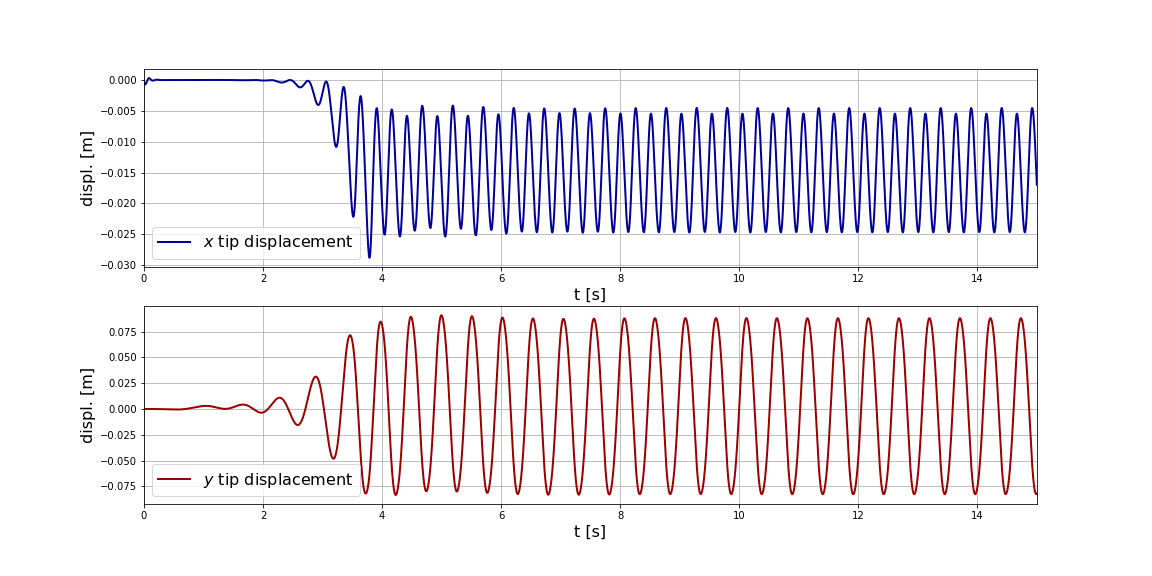
\includegraphics[width=0.98\textwidth, trim=20 20 50 50, clip]{images/FSI2/disp_fsi2.png}
	\caption{FSI2: tip displacement}
	\label{fig:FSI2_displacement}
\end{figure}

Forces are measured on the whole structure on the fluid side, while are measured on the flap in the solid domain. Figure \ref{fig:FSI2_force} shows a detail of $2$ \si{s} of simulation. The difference in \textit{x}-direction represents the drag force on the cylinder.
\begin{figure}[htbp!]
	\centering
	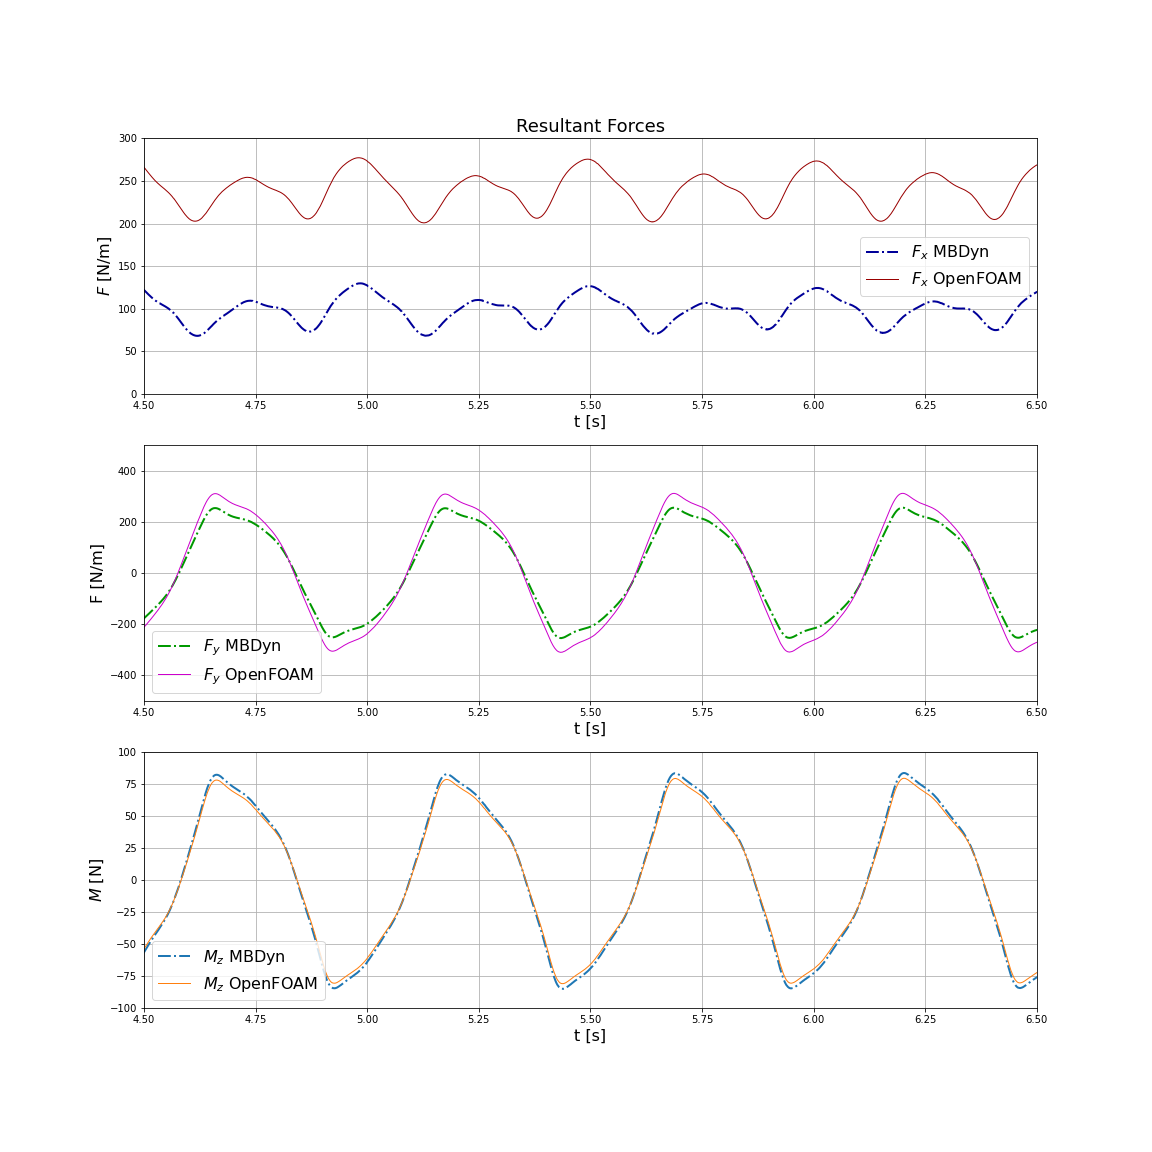
\includegraphics[width=0.98\textwidth, trim=20 100 20 100, clip]{images/FSI2/forces_fsi2.png}
	\caption{FSI2: resultant forces (detail)}
	\label{fig:FSI2_force}
\end{figure}


\begin{figure}[htb]
\centering % <-- added
\begin{subfigure}{0.5\textwidth}
  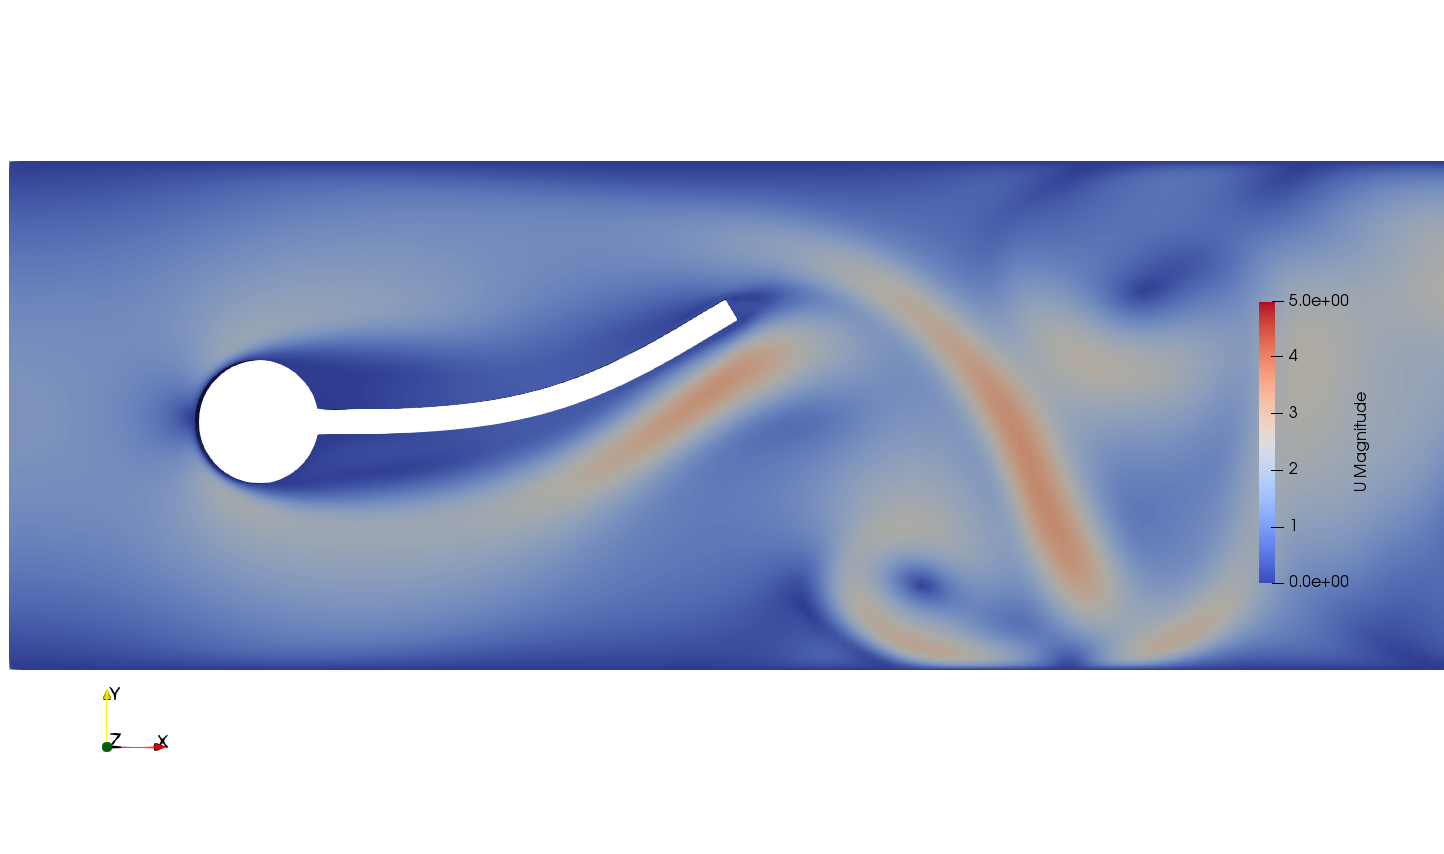
\includegraphics[width=\linewidth, trim=0 120 0 120, clip]{images/FSI2/fsi2_v1.png}
  \caption{t=5.0s velocity}
  \label{fig:fsi2_v1}
\end{subfigure}\hfil % <-- added
\begin{subfigure}{0.5\textwidth}
  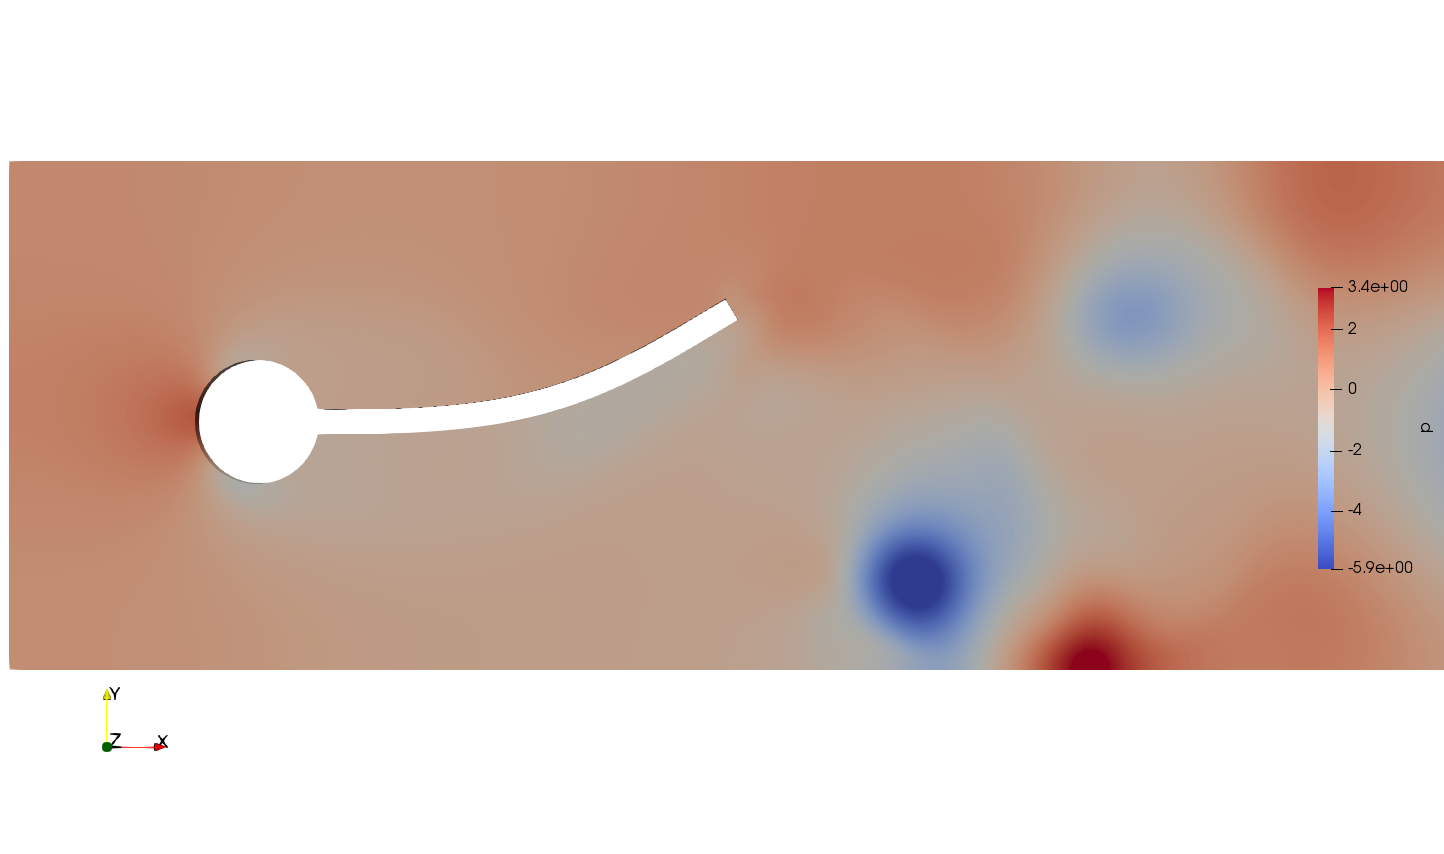
\includegraphics[width=\linewidth, trim=0 120 0 120, clip]{images/FSI2/fsi2_p1.png}
  \caption{t=5.0s pressure}
  \label{fig:fsi2_p1}
\end{subfigure}\hfil % <-- added

\medskip

\begin{subfigure}{0.5\textwidth}
  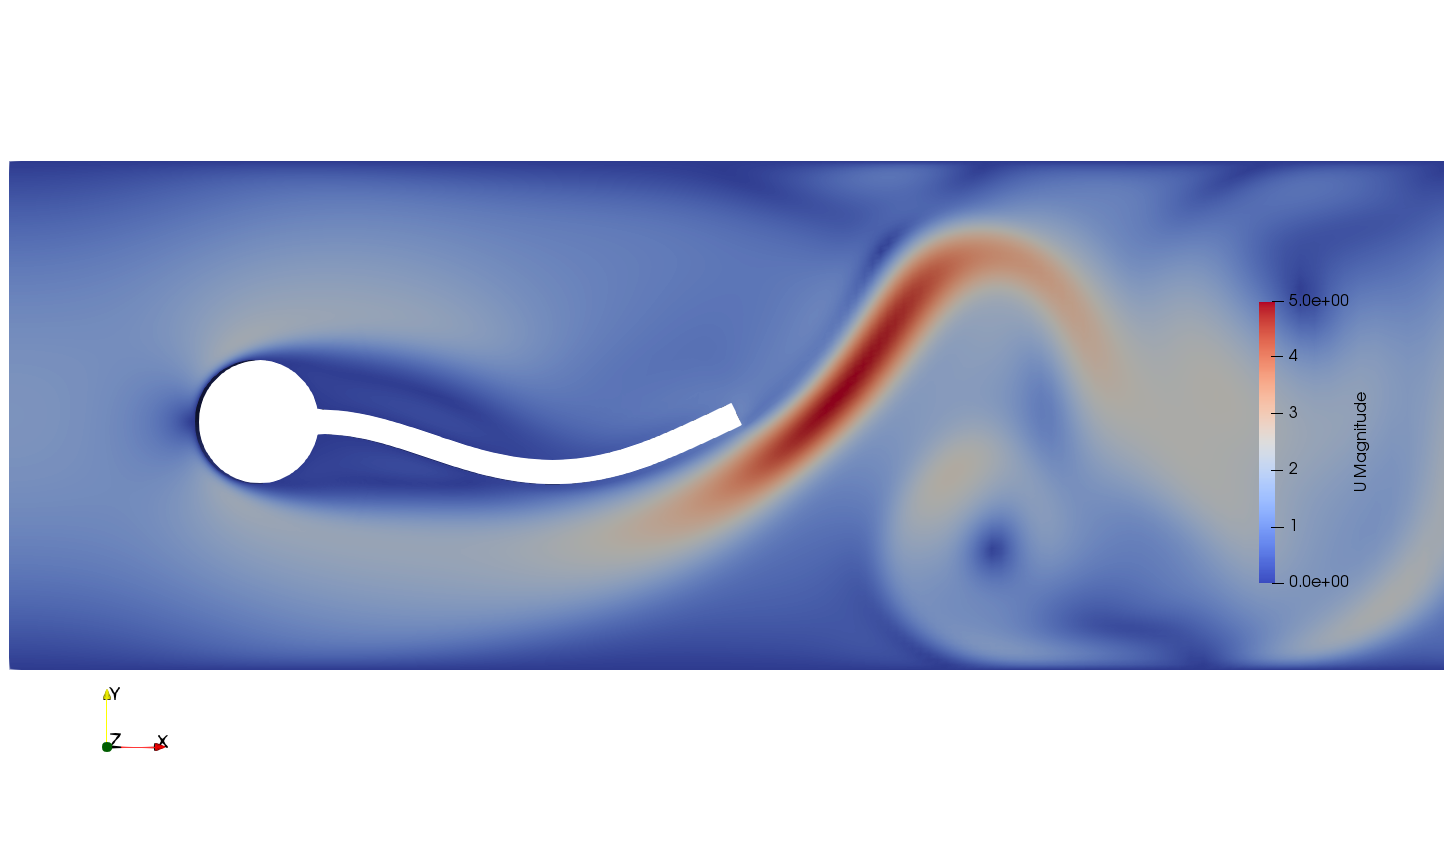
\includegraphics[width=\linewidth, trim=0 120 0 120, clip]{images/FSI2/fsi2_v2.png}
  \caption{t=5.135s velocity}
  \label{fig:fsi2_v2}
\end{subfigure}\hfil % <-- added
\begin{subfigure}{0.5\textwidth}
  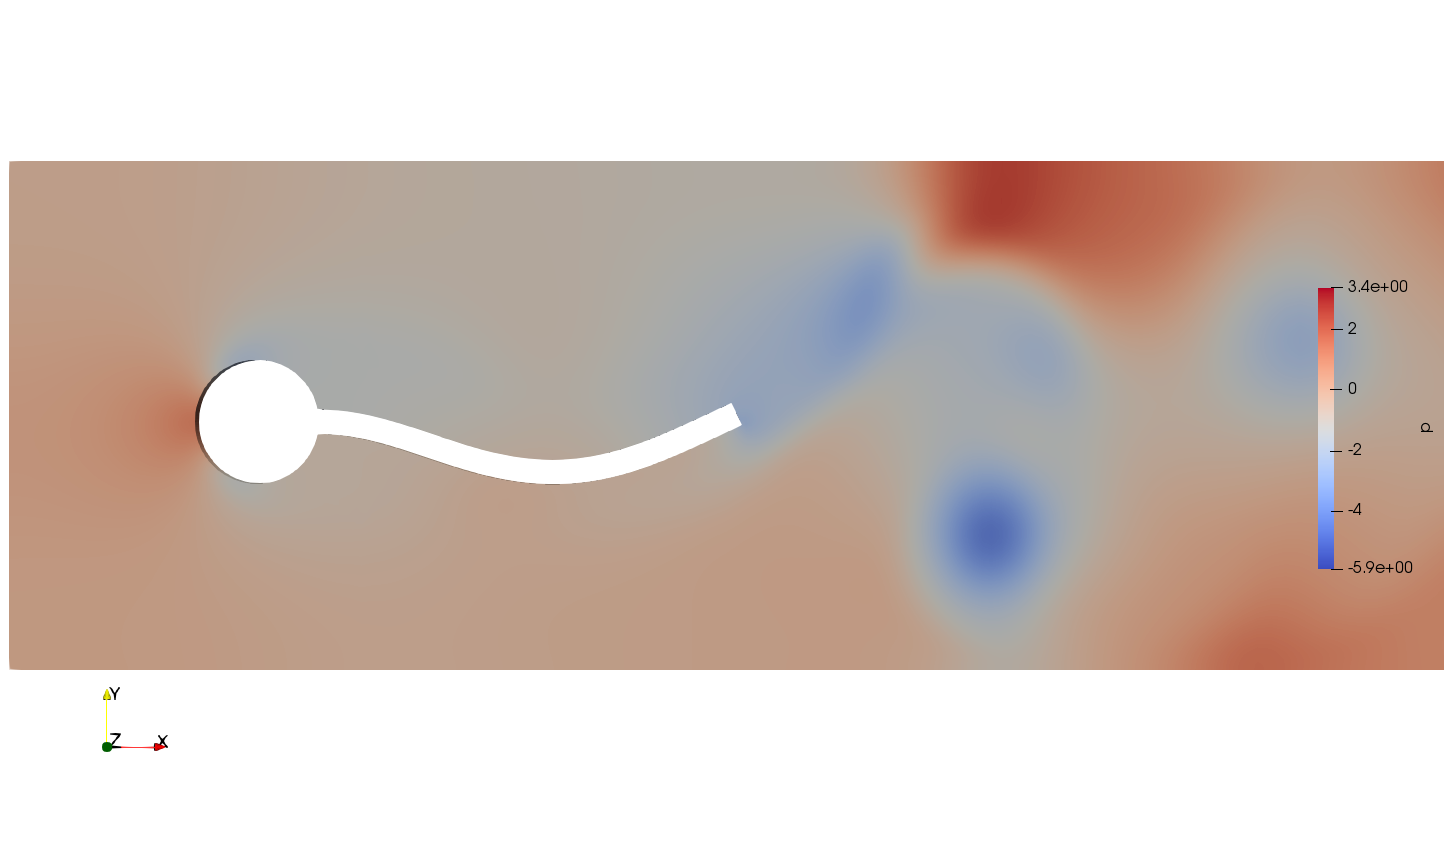
\includegraphics[width=\linewidth, trim=0 120 0 120, clip]{images/FSI2/fsi2_p2.png}
  \caption{t=5.135s pressure}
  \label{fig:fsi2_p2}
\end{subfigure}\hfil % <-- added

\medskip

\begin{subfigure}{0.5\textwidth}
  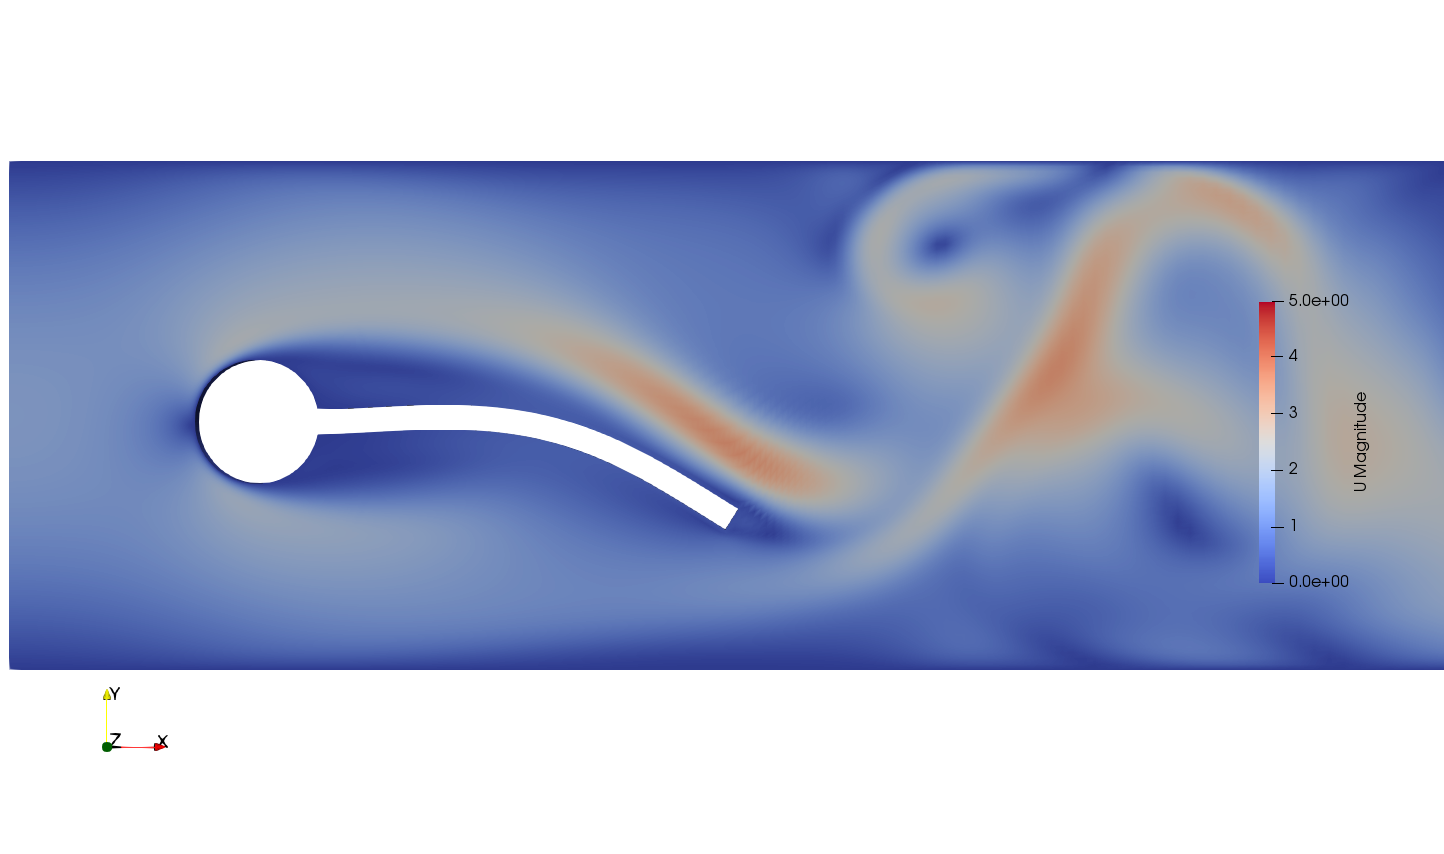
\includegraphics[width=\linewidth, trim=0 120 0 120, clip]{images/FSI2/fsi2_v3.png}
  \caption{t=5.27s velocity}
  \label{fig:fsi2_v3}
\end{subfigure}\hfil % <-- added
\begin{subfigure}{0.5\textwidth}
  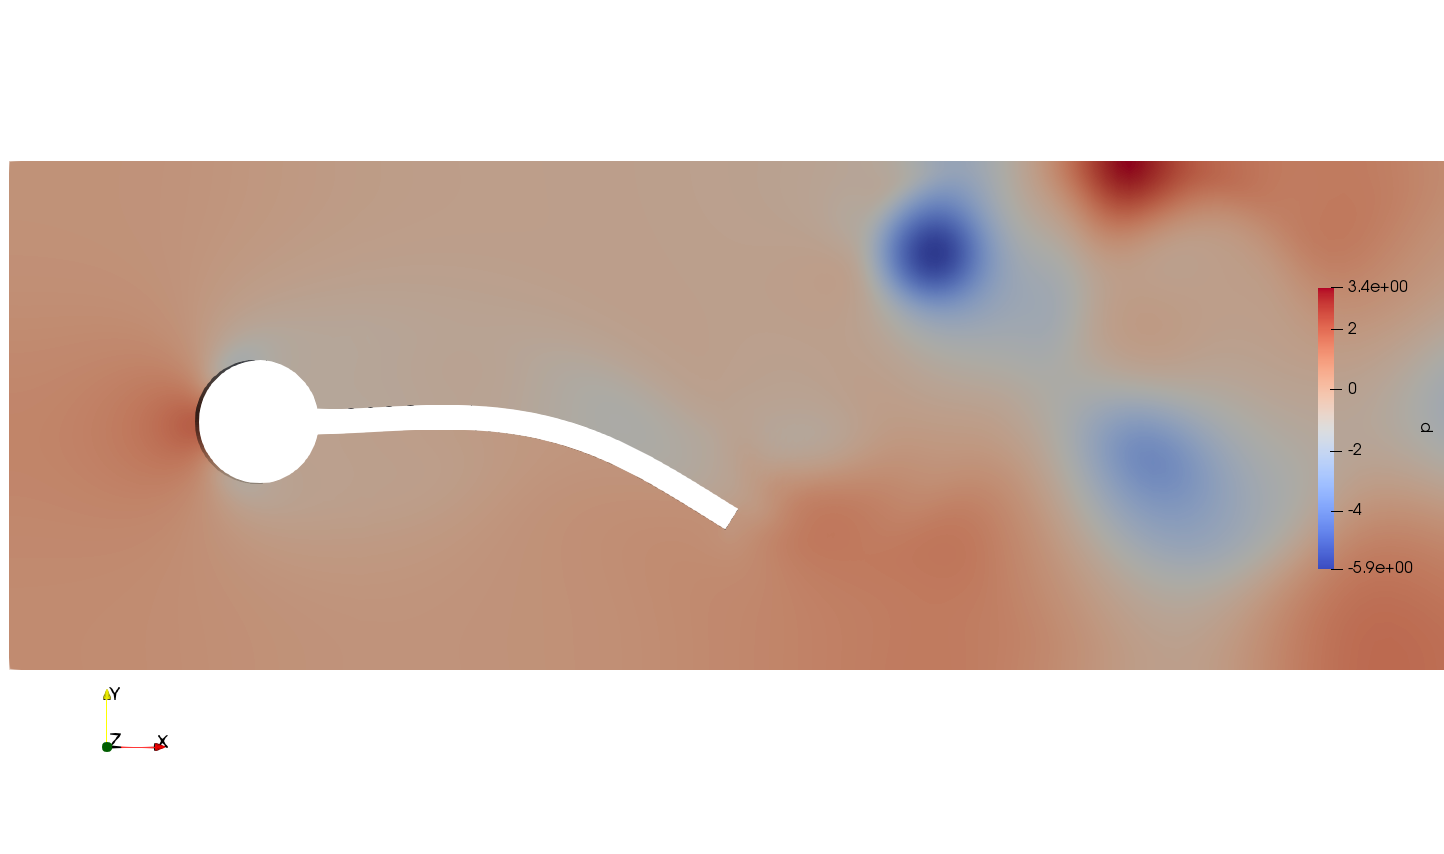
\includegraphics[width=\linewidth, trim=0 120 0 120, clip]{images/FSI2/fsi2_p3.png}
  \caption{t=5.27s pressure}
  \label{fig:fsi2_p3}
\end{subfigure}\hfil % <-- added

\caption{FSI2: fluid solution}
\label{fig:FSI2_sol}
\end{figure}


\hl{Each time step converges with an average of 14.5 iterations, which again confirms the trend of more coupling iterations as the mass number increases.}

\begin{figure}[htbp!]
	\centering
	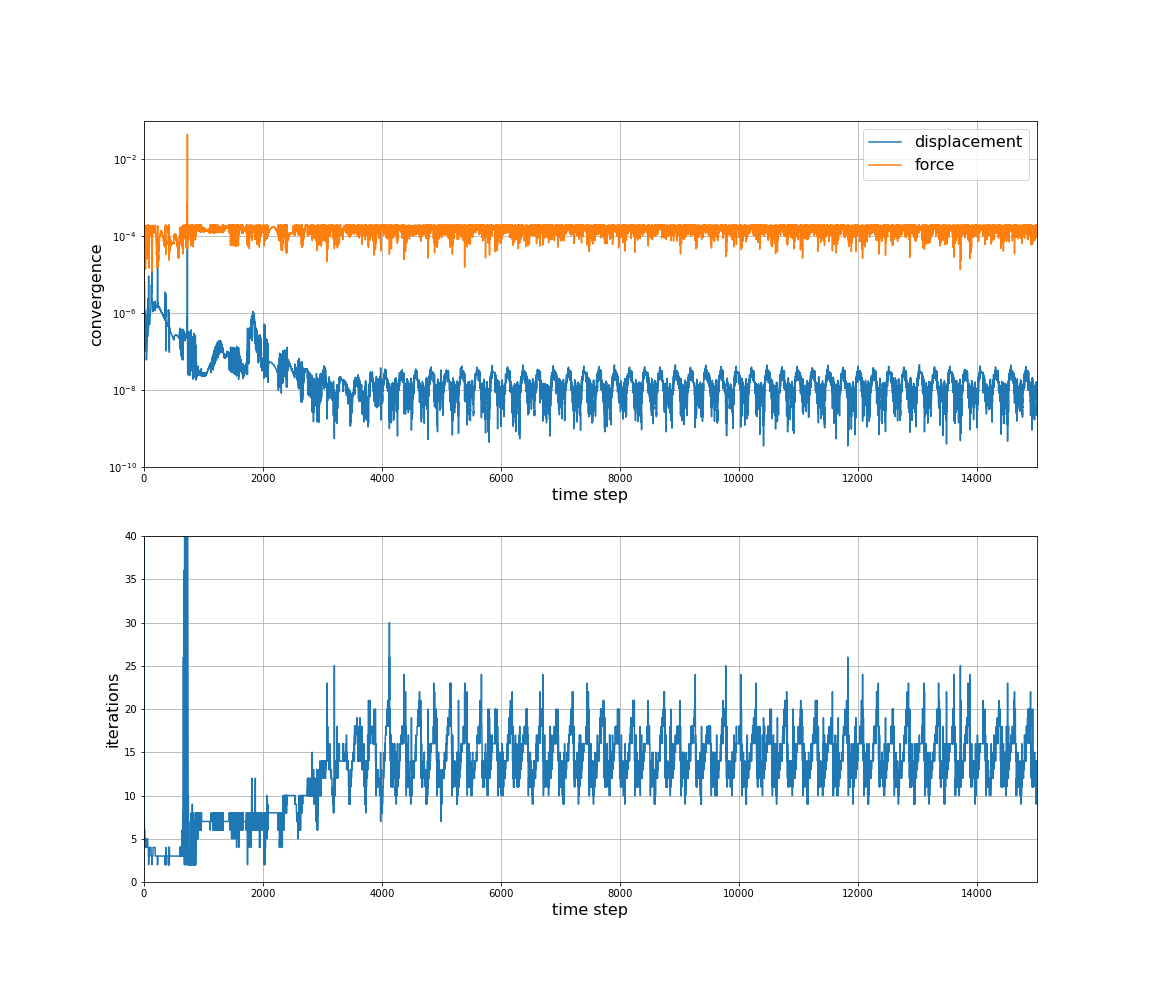
\includegraphics[width=0.95\textwidth, trim=0 80 0 100, clip]{images/FSI2/MBD_iterations_fsi2.png}
	\caption{FSI2: convergence and iterations}
	\label{fig:FSI2_mbd_iter}
\end{figure}

As in the previous examples, the axial, shear and bending moment in each of the MBDyn elements are plotted in Figure \ref{fig:sq_mbd_internal}: in this case a temporal slice of $25s$ has been considered. The values plotted here consider a beam with $2mm$ width: i.e. the thickness of the solid and fluid domains considered in this case.

\begin{figure}[htbp!]
	\centering
	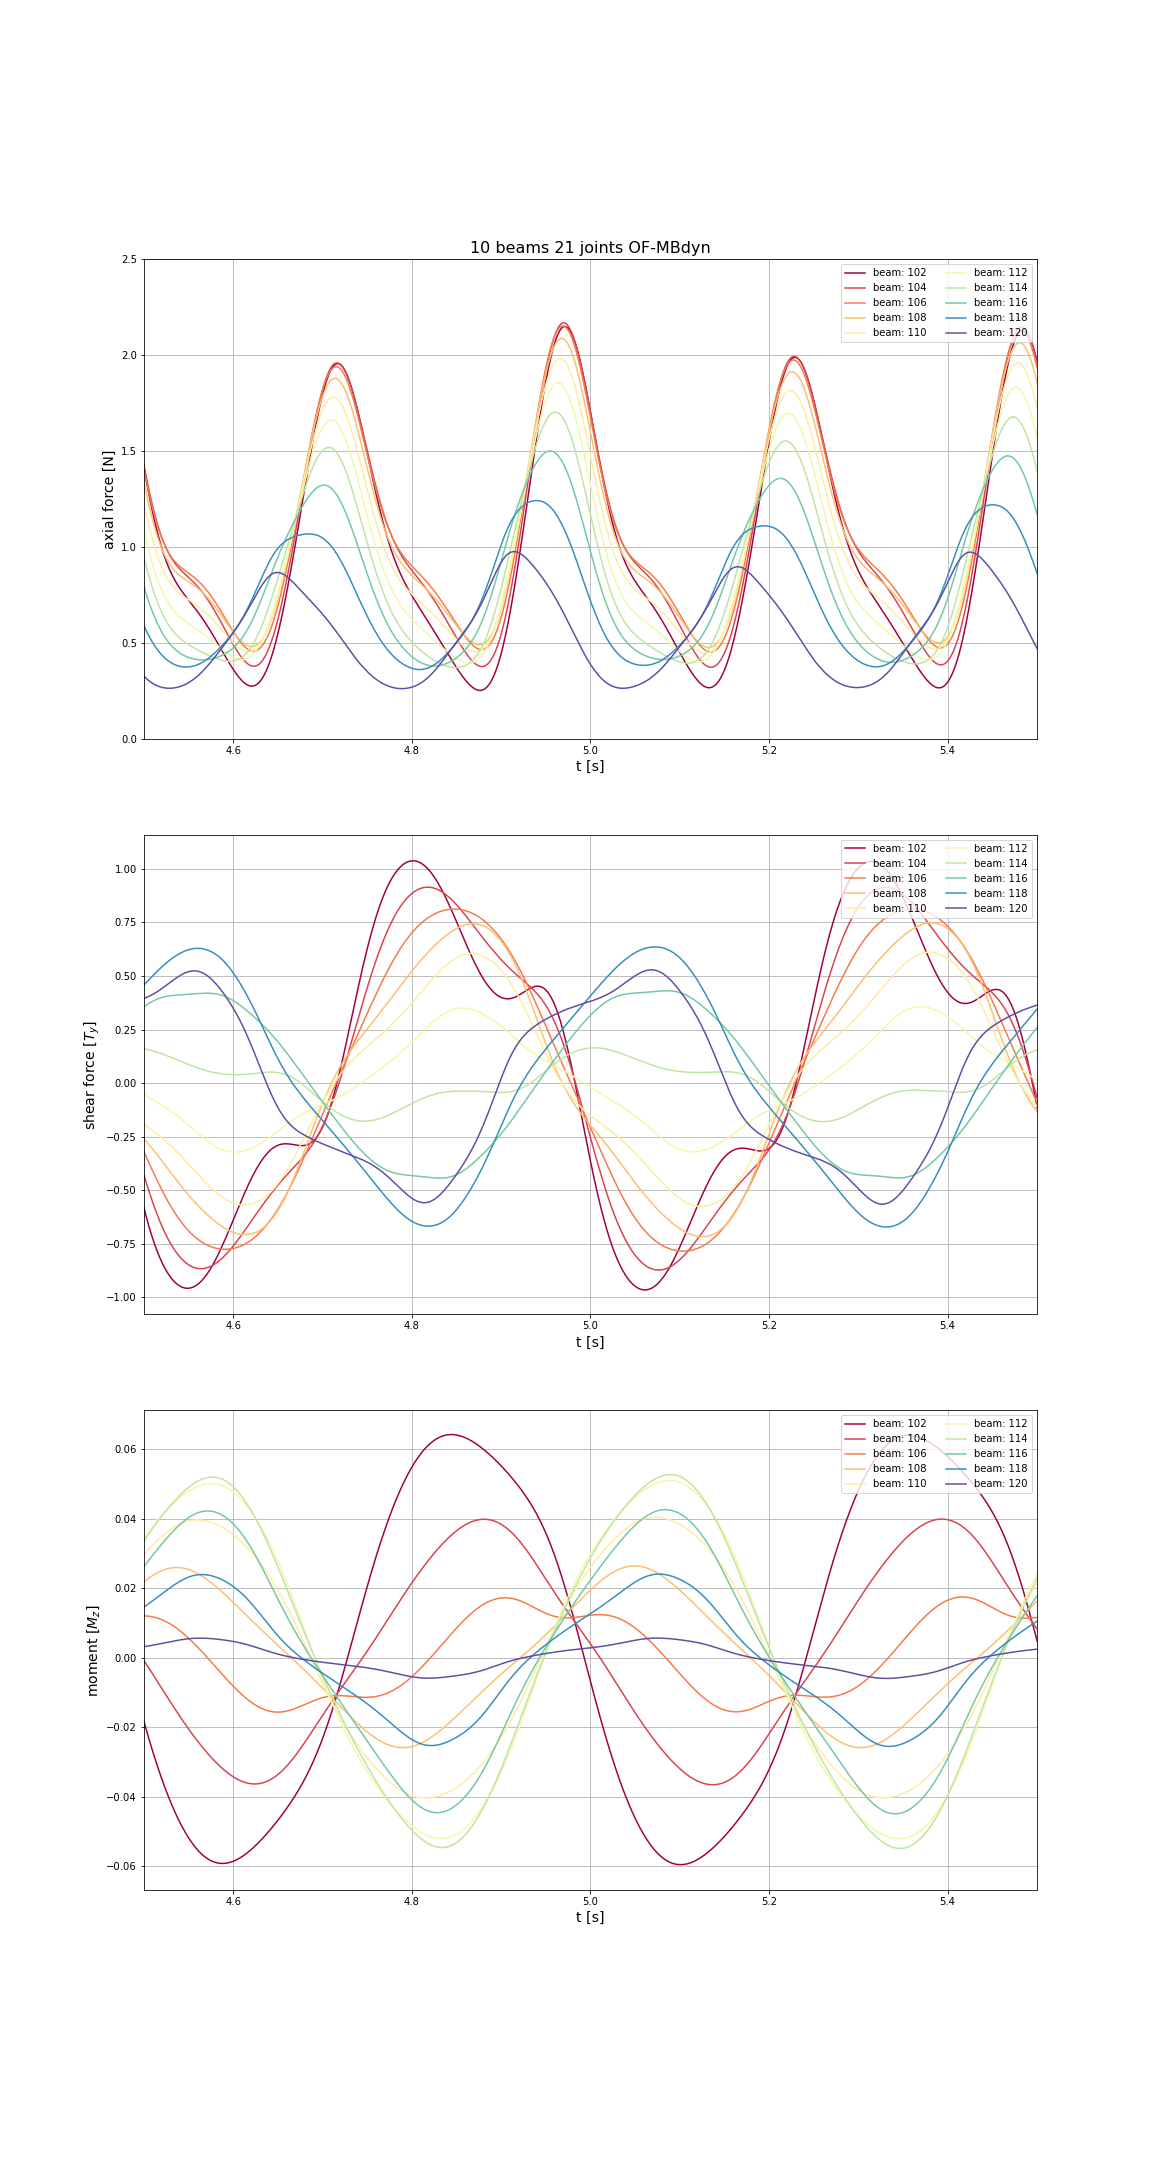
\includegraphics[width=0.92\textwidth, trim=0 230 0 230, clip]{images/FSI2/FSI2_OF-MBDyn_act.png}
	\caption{FSI2: MBDyn internal forces (detail)}
	\label{fig:FSI2_mbd_internal}
\end{figure}


\subsection{Validation}

Turek and Hron benchmarks have been used as a benchmark in many studies considering strongly coupled FSI simulations. 

FSI2 is fully oscillating while the same problem, considering the structure rigid (named CFD2 in \cite{turek2006proposal}) is steady: for this reason it is considered an excellent check for interaction mechanisms \cite{turek2010numerical}.

Besides, FSI2 gives the largest deformation and in some cases it is considered the most difficult of the three benchmarks \cite{richter2015time}, as it gives deformations 2.5 times greater than the flap height.

The comparison of the results can be done in terms of tip displacement and in terms of lift and drag force applied to the whole structure. The results given in the original paper and in a review made by the same authors, together with other studies found in literature are compared to the present study in Table \ref{table:FSI2-results-d} for the data concerning tip displacement, and in Table \ref{table:FSI2-results-f} for the forces applied to the structure.


\begin{table}[!htb]
	\begin{center}
		\begin{tabular}{ l | c c | c c  |  } 
			Study & $d_{x tip}$ [\si{mm}] & f [\si{Hz}] & $d_{y tip}$ [\si{mm}] & f [\si{Hz}] \\ 
			\hline
			\hline
			Benchmark  \cite{turek2006proposal} & $-14.58\pm12.44$ & $3.8$ & $1.23\pm80.6$ & $2.0$     \\
			Turek et al. (2010) \cite{turek2010numerical} & $-14.85\pm12.70$ & $3.86$ & $1.30\pm81.7$ & $1.93$ \\
			Gjertsen \cite{gjertsen2017development} & $-14.83\pm13.11$ & & $1.24\pm81.6$ & \\
			Degroote \cite{degroote2009interface}  & $-14.07\pm12.37$ & $3.7$ & $1.18\pm76.5$ & $1.9$ \\
			Present study & $-14.95\pm9.8$ & $3.87$ & $2.78\pm85.4$ & $1.93$ \\ 
		\end{tabular}
	\end{center}
	\caption{FSI2: comparison of results (displacements)}
	\label{table:FSI2-results-d}
\end{table}

\begin{table}[!htb]
	\begin{center}
		\begin{tabular}{ l | c c | c c  |  } 
			Study & drag [\si{N.m^{-1}}] & f [\si{Hz}] & lift [\si{N.m^{-1}}] & f [\si{Hz}]    \\ 
			\hline
			\hline
			Benchmark  \cite{turek2006proposal} & $208.83\pm73.75$ & $3.8$ & $0.88\pm234.2$ & $2.0$     \\
			Turek et al. (2010) \cite{turek2010numerical} & $215.06\pm77.63$ & $3.86$ & $0.61\pm237.8$ & $1.93$\\   
			Gjertsen \cite{gjertsen2017development} & $161.50\pm73.75$ & & $0.88\pm234.2$ & \\
			Degroote \cite{degroote2009interface}  & $217.52\pm84.65$ & $3.7$ & $-0.74\pm267.6$ & $1.9$ \\
			Present study & $239.13\pm31.9$ & $3.87$ & $2.4\pm217.2$ & $1.93$ \\
		\end{tabular}
	\end{center}
	\caption{FSI2: comparison of results (forces)}
	\label{table:FSI2-results-f}
\end{table}


The study \cite{turek2010numerical} gives 7 different methods and results for FSI1 and FSI3 test cases. In the numerical results it is stated that ``clear differences between the different approaches with regard to accuracy are visible. Particularly for the drag and lift values, which lead to differences of up to order $50\%$, and also for the displacement values which are in the range of $10\%$ errors''.

For the FSI2 test case only the results from the initial Hron and Turek paper \cite{turek2006proposal} and a few others are available.

\hl{ As previously stated, the results for the FSI3 case differ by in
some cases $50\%$ for Drag and Lift. With this in mind, in the FSI2 case I
am off by less then 10% for displacement in x and y direction and for Lift.
While Drag is off by about 50%. It is reasonable to assume that since there
were such differences in the results for different implementations for the FSI3
results, we would expect similar behavior in the FSI2 results.}


\newpage


\section{Turek-Hron FSI3 Benchmark}
\label{sec:FSI1-FSI3}

Omitting for a while the test case named FSI1 as it is not oscillating, the other benchmark proposed in \cite{turek2006proposal}, named FSI3, is very similar to FSI2 with the only different properties shown in Table \ref{table:FSI3-diff}. The corresponding adimensional numbers are given in Table \ref{table:FSI3-adim}. 



\begin{table}[!htb]
	\begin{center}
		\begin{tabular}{ l c l | c | c } 
			parameter & & & FSI2 & FSI3   \\ 
			\hline
			solid density  &  $\rho$ & \si{kg.m^{-3}} & $10000$ & $1000$     \\
			Elastic modulus  & E & \si{Pa} & $1.4\cdot 10^6$ & $5.6\cdot 10^6$   \\
			max flow velocity & $\vec{u}_{max}$ & \si{m.s^{-1}} & $1.5$ & $3$ \\
			mean flow velocity & $\vec{u}$ & \si{m.s^{-1}} & $1$ & $2$  \\
		\end{tabular}
	\end{center}
	\caption{FSI2-FSI3: different parameters}
	\label{table:FSI3-diff}
\end{table}

The 


\begin{table}[!htb]
	\begin{center}
		\begin{tabular}{ l c | c | c} 
			parameter & & FSI2 & FSI3   \\ 
			\hline
			mass number  & $M$ & $0.1$ & $1$     \\
			reduced velocity & $U_R$ &  $8.45 \cdot 10^{-2}$  & $2.67\cdot 10^{-2}$  \\
			Cauchy number  & $C_Y$ & \cellcolor{yellow!25}  $7.14\cdot 10^{-4}$  & \cellcolor{yellow!25} $7.14\cdot 10^{-4}$  \\
			Reynolds number & $Re$ & $100$ & $200$ \\	
		\end{tabular}
	\end{center}
	\caption{FSI2-FSI3: adimensional numbers}
	\label{table:FSI3-adim}
\end{table}


The simulation of FSI3 using MBDyn and OpenFOAM connected with preCICE proved to be an unfeasible task, at least at the time of writing. This same test case is known to work, giving correct results, coupling OpenFOAM and CalculiX as described in the preCICE website\footnote{\href{https://github.com/precice/precice/wiki/Tutorial-for-FSI-with-OpenFOAM-and-CalculiX}{Tutorial-for-FSI-with-OpenFOAM-and-CalculiX}}.
Nevertheless, substituting CalculiX with MBDyn, all other parameters being equal, makes the simulation diverge.

Different approaches have been experimented, acting on each part of the problem. For example:

\begin{itemize}
	\item in the fluid domain:
	\begin{enumerate}
		\item popp
	\end{enumerate}
\end{itemize}



















\section{Sensitivity analysis of FSI1-FSI3 Benchmarks}
\label{sec:FSI3-sensitivity}

\subsection{FSI1 sensitivity Analysis (Re=20)}


\subsection{FSI3 sensitivity Analysis (Re=200)}


\subsection{Sensitivity Analysis at (Re=1000)}

\subsection{Conclusions}
